%%%%%%%%%%%%%%%%%%%%%%%%%%%%%%%%%%%%%%%%%%%%%%%%%%%%%%%%%%%%
%                  TEMPLATE DE TRABALHO
%                  UNESP - SOROCABA
%
%  DADOS DO DOCUMENTO:
%  Altere somente a seção abaixo para reutilizar o modelo.
%%%%%%%%%%%%%%%%%%%%%%%%%%%%%%%%%%%%%%%%%%%%%%%%%%%%%%%%%%%%

\documentclass[a4paper,12pt]{article}


% ==========================================================
%                    DADOS DO DOCUMENTO
% ==========================================================

\newcommand{\Instituicao}{UNESP}
\newcommand{\Campus}{Campus de Sorocaba}
\newcommand{\Instituto}{ICTS -- Instituto de Ciências e Tecnologia}
\newcommand{\Curso}{Engenharia de Controle e Automação}

\newcommand{\Disciplina}{Sistemas Computacionais}
\newcommand{\Titulo}{Desenvolvimento de um \textit{FrontEnd} web para o laboratório LIFS}
\newcommand{\TipoTrabalho}{Trabalho individual 1}

\newcommand{\Autor}{Luiz Henrique Corrêa Monteiro}
\newcommand{\Orientador}{Prof. Dr. Leopoldo A. D. L. Filho}

\newcommand{\EmailAutor}{lh.monteiro@unesp.br}
%\newcommand{\EmailAutorDois}{paulo.ramalho@unesp.br}

\newcommand{\Local}{Sorocaba -- SP}
\newcommand{\Ano}{2026}

\newcommand{\LogoCapa}{2-imagens/image.png}
\newcommand{\ArquivoBibliografia}{referencia.bib}


% ==========================================================
%                    PACOTES
% ==========================================================

% Codificação e idioma
\usepackage[utf8]{inputenc}
\usepackage[T1]{fontenc}
\usepackage[portuguese]{babel}

% Fonte
\usepackage{times}

% Margens
\usepackage[
a4paper,
left=3cm,
right=2cm,
top=3cm,
bottom=2cm
]{geometry}

% Imagens
\usepackage{graphicx}
\graphicspath{{2-imagens/}}

% Matemática
\usepackage{
	amsmath,
	amssymb,
	amsfonts,
	amsthm,
	amscd,
	latexsym
}

% Formatação
\usepackage{titlesec}
\usepackage{fontawesome5}
\usepackage{indentfirst}
\usepackage{setspace}
\usepackage{enumitem}
\usepackage{multicol}
\usepackage{multirow}
\usepackage{array}
\usepackage{float}
\usepackage{caption}
\usepackage{subcaption}
\usepackage{tcolorbox}
\usepackage{tabularx}
\usepackage{tikz}
\usetikzlibrary{arrows.meta, positioning, shapes.geometric}
\usepackage{array}
\usepackage{ragged2e}
\usepackage{booktabs}
\usepackage{longtable}

% Outros
\usepackage{fancyhdr}
\usepackage{hyperref}
\usepackage{nameref}
\usepackage{etoolbox}
\usepackage{pdflscape}
\usepackage{cancel}
\usepackage{verbatim}
\usepackage{csquotes}
\usepackage{algorithm2e}
\usepackage{longtable}

% Código
\usepackage{listings}
\usepackage{xcolor}
\usepackage{colortbl}


\definecolor{iaGeracao}{RGB}{218,235,247} \definecolor{iaCorrecao}{RGB}{252,229,205} \definecolor{iaRefinamento}{RGB}{220,240,220} \definecolor{iaAcessibilidade}{RGB}{231,222,245} \definecolor{iaReestruturacao}{RGB}{255,242,190} \definecolor{iaSemEvidencia}{RGB}{235,235,235}
% Cores
\definecolor{githubcolor}{HTML}{24292F}
\definecolor{metricscolor}{HTML}{7B2CBF}
\definecolor{websitecolor}{HTML}{2D6A4F}
% Cores do histórico Git
\definecolor{terminalbg}{RGB}{24,26,27}
\definecolor{terminaltext}{RGB}{220,220,220}
\definecolor{gitgreen}{RGB}{80,200,120}
\definecolor{gitred}{RGB}{255,100,100}
\definecolor{gitpurple}{RGB}{190,130,255}
\definecolor{gitorange}{RGB}{255,170,70}
\definecolor{gitblue}{RGB}{100,170,255}
\definecolor{gitcyan}{RGB}{80,210,210}
\definecolor{gitgray}{RGB}{150,160,165}
\definecolor{gitbranch}{RGB}{255,210,80}

\lstdefinelanguage{GitHistory}{
	morekeywords={
		feat,
		fix,
		style,
		perf,
		docs,
		chore,
		refactor,
		Feature,
		STYLE
	},
	sensitive=true,
}

\lstdefinestyle{gitstyle}{
	language=GitHistory,
	backgroundcolor=\color{terminalbg},
	basicstyle=\ttfamily\small\color{terminaltext},
	keywordstyle=\color{gitgreen}\bfseries,
	commentstyle=\color{gitgray},
	stringstyle=\color{gitblue},
	columns=fullflexible,
	keepspaces=true,
	showstringspaces=false,
	breaklines=true,
	breakatwhitespace=false,
	frame=single,
	framerule=0.6pt,
	rulecolor=\color{black!50},
	xleftmargin=0.3cm,
	xrightmargin=0.3cm,
	aboveskip=10pt,
	belowskip=10pt,
	tabsize=4
}

\lstdefinelanguage{CSS}{
	morekeywords={
		display, position, top, left, right, bottom,
		width, height, max-width, min-width,
		margin, padding, gap,
		grid-template-columns, grid-template-rows,
		flex-direction, align-items, justify-content,
		font-size, font-family, font-weight,
		color, background, border,
		box-sizing, z-index,
		overflow, transition, animation,
		outline, outline-offset,
		order, scroll-behavior
	},
	sensitive=true,
	morecomment=[s]{/*}{*/},
	morestring=[b]"
}

% ==========================================================
%                    BIBLIOGRAFIA
% ==========================================================

\usepackage[
backend=biber,
style=abnt
]{biblatex}

\addbibresource{\ArquivoBibliografia}


% ==========================================================
%                    ESPAÇAMENTO
% ==========================================================

\titlespacing*{\section}
{0pt}
{-5pt}
{5pt}

\titlespacing*{\subsection}
{0pt}
{-5pt}
{5pt}


% ==========================================================
%                    CORES DOS CÓDIGOS
% ==========================================================

\definecolor{backcolour}{rgb}{0.95,0.95,0.92}
\definecolor{codegreen}{rgb}{0,0.6,0}
\definecolor{codegray}{rgb}{0.5,0.5,0.5}
\definecolor{codepurple}{rgb}{0.58,0,0.82}
\definecolor{bluekeyword}{rgb}{0.13,0.13,1}
\definecolor{typecolor}{rgb}{0.17,0.57,0.68}
\definecolor{macrocolor}{rgb}{0.5,0.0,0.0}


% ==========================================================
%                    CONFIGURAÇÃO DO LISTINGS
% ==========================================================

\lstset{
	language=C++,
	backgroundcolor=\color{backcolour},
	commentstyle=\color{codegreen},
	keywordstyle=\color{bluekeyword}\bfseries,
	numberstyle=\tiny\color{codegray},
	stringstyle=\color{codepurple},
	basicstyle=\ttfamily\scriptsize,
	breakatwhitespace=false,
	breaklines=true,
	keepspaces=true,
	numbers=left,
	numbersep=5pt,
	showspaces=false,
	showstringspaces=false,
	showtabs=false,
	tabsize=4,
	captionpos=b
}

% Palavras adicionais
\lstset{
	morekeywords={
		uint8_t,
		size_t,
		esp_err_t,
		ESP_RETURN_ON_FALSE,
		i2c_master_transmit_receive,
		i2c_master_transmit,
		static_cast
	}
}


% ==========================================================
%                    HYPERLINKS
% ==========================================================

\hypersetup{
	hidelinks
}


% ==========================================================
%                    INÍCIO DO DOCUMENTO
% ==========================================================

\begin{document}
	
	\pagenumbering{arabic}
	
	
	% ==========================================================
	%                         CAPA
	% ==========================================================
	
	\begin{titlepage}
		
		\begin{center}
			
			\includegraphics[
			width=0.8\linewidth
			]{\LogoCapa}
			
			\vspace*{1cm}
			
			\textbf{\Large \Campus}\\
			\textbf{\Large \Instituto}\\[3cm]
			
			\large{\TipoTrabalho}\\[2cm]
			
			{\large\textbf{\Disciplina}}\\[4cm]
			
			\vfill
			
			\Large\textbf{Discente: \Autor}\\
			\textbf{Orientador: \Orientador}\\[3cm]
			
			\Local\\
			\Ano
			
		\end{center}
		
	\end{titlepage}
	
	
	% ==========================================================
	%                     FOLHA DE ROSTO
	% ==========================================================
	
	\begin{titlepage}
		
		\begin{center}
			
			\vspace*{1cm}
			
			\textbf{\Autor}\\[2cm]
			
			\large\textbf{\Titulo}\\[3cm]
			
			Trabalho apresentado ao \Instituto\ da \Instituicao,
			como parte dos requisitos para a conclusão da disciplina
			de \Disciplina.\\[2cm]
			
			Orientador: \Orientador\\[3cm]
			
			\textit{E-mail do aluno autor:}\\
			
			\texttt{\EmailAutor}\\
			%\texttt{\EmailAutorDois}\\[3cm]
			\vfill
			\Local\\
			\Ano
			
		\end{center}
		
	\end{titlepage}
	
	
	% ==========================================================
	%                         SUMÁRIO
	% ==========================================================
	
	\tableofcontents
	
	\newpage
	
	
	% ==========================================================
	%                        CONTEÚDO
	% ==========================================================
	
	% Introdução

\section{Introdução}
%\addcontentsline{toc}{chapter}{Introdução} % Adiciona "Introdução" ao sumário
O presente trabalho aborda o desenvolvimento de uma interface web para o Laboratório de Investigação de Filmes Semicondutores (LIFS), com o objetivo de centralizar informações que anteriormente se encontravam dispersas e facilitar o acesso ao conteúdo do laboratório. A proposta surgiu a partir da necessidade de disponibilizar, em um único ambiente, informações sobre o grupo, seus membros, equipamentos, trabalhos acadêmicos e atividades.

O projeto foi desenvolvido considerando principalmente pesquisadores, estudantes e possíveis parceiros externos, buscando uma interface simples, responsiva e acessível. Além da implementação das páginas e funcionalidades previstas, foram realizadas avaliações de desempenho, acessibilidade, responsividade e compatibilidade, permitindo verificar o comportamento da aplicação e identificar pontos que ainda podem ser aprimorados.

Os links e arquivos podem ser obtidos, clicando nos seguintes botões. 

\begin{center}
	
	\noindent
	\begin{minipage}[c]{0.30\textwidth}
		\centering
		\href{https://github.com/rick-12q/SCOM_1_LIFS_SITE}{
			\textcolor{githubcolor}{
				\Large\faGithub
			}
			\\[5pt]
			\textbf{\textcolor{githubcolor}{Repositório}}
		}
	\end{minipage}
	\hfill
	\begin{minipage}[c]{0.30\textwidth}
		\centering
		\href{https://github.com/rick-12q/SCOM_1_LIFS_SITE/blob/main/metricas.zip}{
			\textcolor{metricscolor}{
				\Large\faChartLine
			}
			\\[5pt]
			\textbf{\textcolor{metricscolor}{Métricas}}
		}
	\end{minipage}
	\hfill
	\begin{minipage}[c]{0.30\textwidth}
		\centering
		\href{https://rick-12q.github.io/SCOM_1_LIFS_SITE/}{
			\textcolor{websitecolor}{
				\Large\faGlobe
			}
			\\[5pt]
			\textbf{\textcolor{websitecolor}{Website}}
		}
	\end{minipage}
	
\end{center}

\newpage
	
	
%%======%%======%0%======%%=======%%
\vspace{5mm}
\section{Problema e público alvo}
\label{sec:Publico}
%\addcontentsline{toc}{chapter}{Objetivos}

%%======%%======%0%======%%=======%%

O desenvolvimento do Site \textbf{Lab-LIFS} carrega consigo uma notável importância prática, uma vez que o grupo nunca possuiu de fato uma interface web que permitisse a integração do lab. com pessoas externas do circulo de convivência dos internos. O laboratório, atualmente, possui caráter de desenvolver pesquisas e compartilhar o uso de equipamentos presentes nas dependências do grupo. Tendo isso em vista, o aluno autor, por integrar o grupo de pesquisa, entendeu a relevância e aplicação prática de tal desenvolvimento. 

O objetivo foi portanto, criar uma interface web que permitisse de tal modo que, informações as quais antes estavam soltas, desconexas e muitas vezes difusas, agora estarão concentradas dentro de uma mesma central, de modo a facilitar bilateralmente as interações, e tornar inclusive o grupo de pesquisa mais profissional. A ideia, ao ser transmitida para o professor Dr. José R. R. Bortoleto, chefe do laboratório, foi recebida com grande alegria, entusiasmo e disposição, evidenciando que a ideia de fato sanaria um problema que é um antigo conhecido do grupo. O projeto buscou a realização das seguintes funções:
\begin{itemize}
	\item Agendamento de equipamentos e máquinas presentes no lab.;
	\item Visualização de notícias recentes e conquistas do grupo;
	\item Acesso ao acervo público de artigos, congressos, etc;
	\item Contato com alunos e professores, de modo a divulgar os trabalhos e conectar possíveis parceiros ou novos membros.
\end{itemize}


Para tal, já era entendido pelo aluno autor, que muitos usuários seriam pessoas que não são da área temática de tecnologia, mas sim na área de física ou materiais, logo, o objetivo sempre foi desenvolver uma interface responsiva, simples e prática, visto que o público alvo é outros pesquisadores da área, alunos e empresas que buscam parcerias em instituições de pesquisa tal qual a UNESP. Portanto, foi desenvolvido por meio do \textit{software} \textit{excalidraw}, um \textit{wireframe} para o projeto, de modo a melhor adequar e pegar outras referências, criando algo funcional, esteticamente agradável e moderno. A Figura \ref{fig:wireframeproject} mostra o \textit{wireframe} feito. 
\begin{figure}[H]
	\centering
	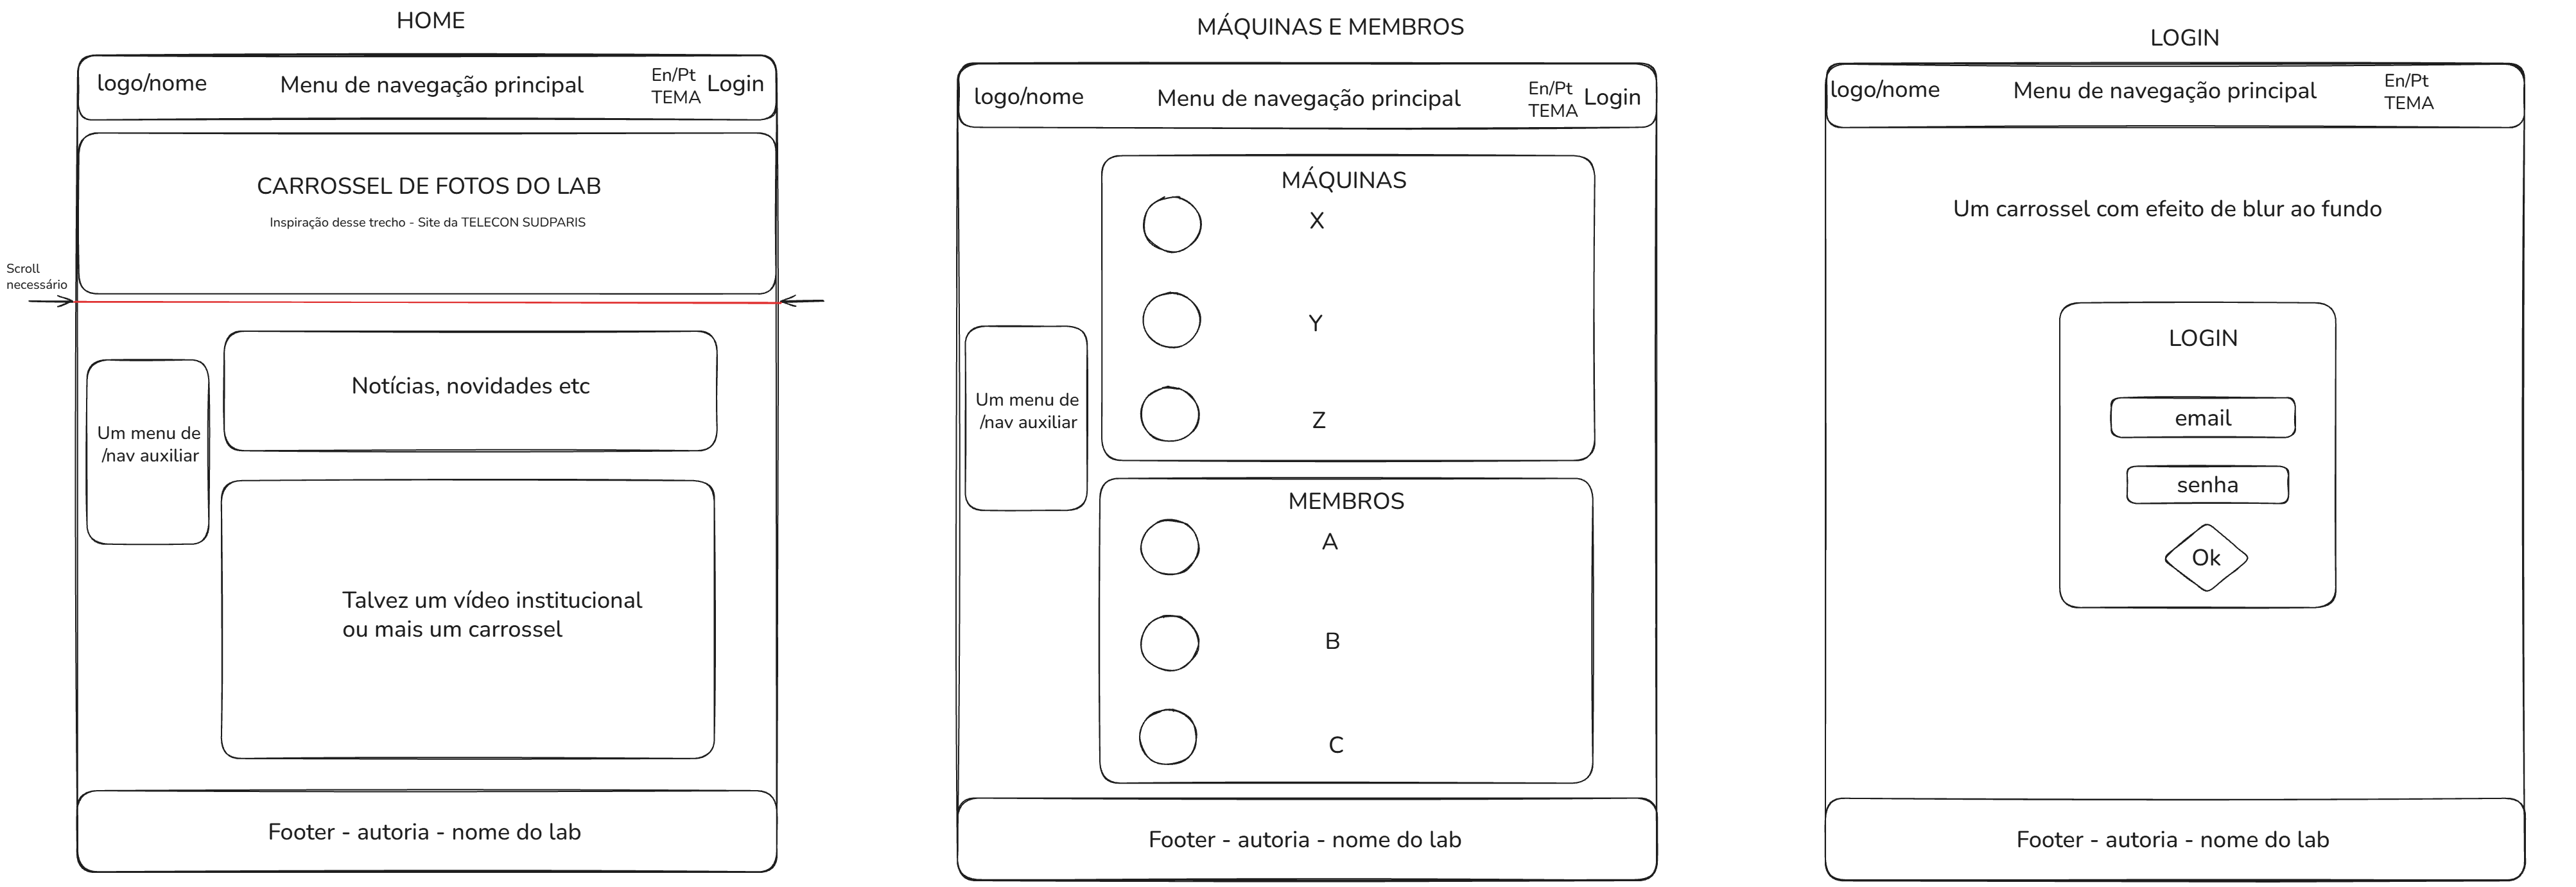
\includegraphics[width=1\linewidth]{2-imagens/wireframe_project}
	\caption{Esboço da interface idealizada para o projeto em questão.\\Fonte: O autor, 2026.}
	\label{fig:wireframeproject}
\end{figure}

	
	
%%======%%======%0%======%%=======%%
\vspace{5mm}
\section{Requisitos do sistema}
\label{sec:Requisitos}
%\addcontentsline{toc}{chapter}{Objetivos}

%%======%%======%0%======%%=======%%

Uma vez bem compreendido o problema a ser sanado e o público alvo, foi necessário listar todos os requisitos do sistema a ser desenvolvido. Para tal, foi feita uma pesquisa em campo, onde o aluno autor se dispôs a conversar com três Professores Pesquisadores, da área de materiais, para melhor compreender as reais necessidades, os professores em questão foram:
\begin{itemize}
	\item Prof. Dr. José R. R. Bortoleto (UNESP);
	\item Prof. Me. Paulo Silas Oliveira (Instituto Federal);
	\item Prof. Dr. Raul Ramos (UNICAMP).
\end{itemize}
As respostas obtidas foram organizadas e sintetizadas a seguir.
\vspace{5mm}
\subsection{Conteúdo esperado para a página inicial}

Quando questionados sobre quais informações deveriam ser apresentadas na página inicial do sistema, foram identificadas três expectativas principais:

\begin{enumerate}
	\item \textbf{Apresentação do laboratório:} disponibilizar uma página introdutória que apresente o laboratório, sua finalidade, suas áreas de atuação e suas principais características;
	
	\item \textbf{Pesquisas e frentes de trabalho:} apresentar as principais linhas de pesquisa, projetos e frentes de trabalho desenvolvidas pelo grupo;
	
	\item \textbf{Panorama das atividades do grupo:} disponibilizar uma síntese das atividades realizadas, contemplando acontecimentos recentes, projetos em andamento, resultados e demais novidades relevantes.
\end{enumerate}

Dessa forma, observa-se que a página inicial é percebida como um meio de divulgação e contextualização das atividades desenvolvidas pelo laboratório.
\vspace{5mm}
\subsection{Funcionalidades esperadas para o sistema}

Em relação às funcionalidades esperadas, as respostas indicaram a necessidade de uma plataforma que além de apresentar informações institucionais também ofereça recursos para integração, organização e gerenciamento das atividades do grupo. Entre as principais funcionalidades mencionadas, destacam-se:

\begin{enumerate}
	\item \textbf{Integração entre membros e público externo:} possibilitar a comunicação e a aproximação entre os integrantes do grupo e pessoas externas ao laboratório, facilitando o acesso às informações e aos trabalhos desenvolvidos;
	
	\item \textbf{Agendamento e gerenciamento de recursos:} permitir a realização de agendamentos, a consulta de disponibilidade e a organização do uso dos recursos e equipamentos do laboratório;
	
	\item \textbf{Repositório de trabalhos:} disponibilizar um espaço destinado ao armazenamento e à consulta de trabalhos acadêmicos, projetos, publicações e demais produções desenvolvidas pelo grupo;
	
	\item \textbf{Gerenciamento de reagentes e insumos:} possibilitar a consulta às informações relacionadas aos reagentes e materiais disponíveis no laboratório;
	
	\item \textbf{Informações sobre máquinas e equipamentos:} apresentar os equipamentos disponíveis, suas características e, quando aplicável, sua disponibilidade para utilização;
	
	\item \textbf{Divulgação de novidades:} disponibilizar informações sobre acontecimentos recentes, atividades, projetos, resultados e demais novidades relacionadas ao grupo.
\end{enumerate}

A partir dessas respostas, verifica-se uma expectativa de que o sistema atue como uma plataforma integrada de informações e gerenciamento, reunindo em um único ambiente tanto os aspectos institucionais e acadêmicos do laboratório quanto os recursos necessários à organização de suas atividades, tais dados foram abstraídos pelo aluno autor, e pode ser desenvolvida a seguinte lista de requisitos ligados a parte técnica do projeto:
\begin{itemize}
	\item ser responsivo;
	\item possuir contraste adequado;
	\item utilizar estrutura HTML semântica;
	\item funcionar nos navegadores exigidos;
	\item apresentar desempenho adequado
	\item ser simples de usar.
	\item apresentar informações do laboratório;
	\item disponibilizar trabalhos;
	\item permitir agendamento;
\end{itemize}

	
	%%======%%======%0%======%%=======%%
\vspace{5mm}
\section{Processo de projeto}
%\addcontentsline{toc}{chapter}{Resultados e discussões}

%%======%%======%0%======%%=======%%

Para satisfazer as necessidades presentes na Seção \ref{sec:Publico} e \ref{sec:Requisitos}, foi necessário dividir o projeto em 5  grandes etapas, as quais foram realizadas, em boa parte do tempo, sequencialmente.
\vspace{5mm}
\subsection{Levantamento inicial}
Em primeiro passo, foi realizado o levantamento inicial de estruturas, modelos e estilos que satisfizessem as questões previamente discutidas na Seção \ref{sec:Requisitos}. Para tal, foi feito um levantamento em diversos \textit{websites}, desde instituições de ensino nacionais e internacionais, até empresas de usinagem pesada. Os modelos que mais se aproximaram das ideias discutidas previamente foram os seguintes sites:\\
\href{https://www.telecom-sudparis.eu/en/}{\textcolor{red}{site 1}}, que pertence a universidade Francesa Telecom sudParis;\\
\href{https://nupem.com.br/especialidades/medicina-estetica-2/}{\textcolor{blue}{site 2}}, que pertence a uma médica. 

\vspace{5mm}
\subsection{Definição das páginas}
Foram definidas então as páginas presentes no trabalho, de modo a atender as solicitações, gerar um visual simples e harmônico. Para tal, a Tabela \ref{tab:paginas}, explicita as páginas criadas e seu respectivo conteúdo. 
\begin{table}[H]
	\centering
	\caption{Páginas desenvolvidas para o sistema e seus respectivos conteúdos.}
	\label{tab:paginas}
	\renewcommand{\arraystretch}{1.4}
	\begin{tabularx}{\textwidth}{>{\raggedright\arraybackslash}p{0.22\textwidth} X}
		\hline
		\textbf{Página} & \textbf{Conteúdo} \\
		\hline
		Inicio & Apresentação do laboratório, notícias recentes e panorama geral das atividades desenvolvidas pelo grupo. \\[2pt]
		
		Repositório & Exposição dos trabalhos, artigos, anais de congressos e demais produções acadêmicas do grupo. \\[2pt]
		
		Máquinas & Exposição dos equipamentos disponíveis no laboratório, bem como possibilidade de consulta à disponibilidade e realização de agendamentos. \\[2pt]
		
		Membros & Exposição dos membros do laboratório, suas respectivas funções e opções de contato. \\[2pt]
		
		Entrar & Tela destinada à autenticação dos usuários no sistema. \\[2pt]
		
		Adicionar\_trabalho & Funcionalidade disponível após a realização do login, permitindo a inserção de novos trabalhos no repositório. \\
		\hline
	\end{tabularx}
\end{table}

\vspace{5mm}
\subsection{Evolução}
Após as definições de requisitos, estilos e funcionalidades, a parte do código começou a ser estruturada. Para tal, foi utilizado o ambiente do \textit{Visual Studio Code} (VScode), além do editor padrão, foram usadas como auxílio, as extensões:
\begin{itemize}
	\item Prettier;
	\item Material Icon Theme;
	\item Auto Rename Tag;
	\item Live Server.
\end{itemize}

A evolução estrutural do código foi realizada de maneira que, as evoluções convergissem para o modelo de interface esperada. Toda a evolução do código, pode ser observada no repositório criado no \href{https://github.com/rick-12q/SCOM_1_LIFS_SITE}{\textit{\textcolor{blue}{Git}\textcolor{purple}{Hub}}}. O projeto seguiu a seguinte sequência lógica:
	%--Tentar fazer essa bomba
\begin{figure}[H]
	\centering
	
	\begin{tikzpicture}[
		box/.style={
			rectangle,
			rounded corners=3pt,
			draw,
			text width=3.2cm,
			minimum height=1.25cm,
			align=center,
			font=\small,
			inner sep=6pt
		},
		arrow/.style={
			-{Stealth[length=2.2mm]},
			thick
		}
		]
		
		% frst line
		\node[box] (estrutura) at (0,0) {
			\textbf{Estruturação}\\[2pt]
			Criação das pastas e arquivos essenciais
		};
		
		\node[box] (html) at (4.2,0) {
			\textbf{Estrutura HTML}\\[2pt]
			Definição da estrutura básica das páginas
		};
		
		\node[box] (css) at (8.4,0) {
			\textbf{Identidade visual}\\[2pt]
			Desenvolvimento dos estilos e padrões visuais
		};
		
		\node[box] (desenvolvimento) at (12.6,0) {
			\textbf{Desenvolvimento}\\[2pt]
			Criação dos arquivos HTML, CSS e JS por página
		};
		
		% sgnd line
		\node[box] (refinamento) at (12.6,-3.0) {
			\textbf{Refinamento}\\[2pt]
			Revisão e aprimoramento do código com auxílio de IA
		};
		
		\node[box] (melhorias) at (8.4,-3.0) {
			\textbf{Melhorias}\\[2pt]
			Novas funcionalidades e ajustes pontuais com IA
		};
		
		\node[box] (correcoes) at (4.2,-3.0) {
			\textbf{Correções}\\[2pt]
			Identificação e correção de erros (\textit{bugs}) com ajuda de IA
		};
		%--
		\draw[arrow] (estrutura) -- (html);
		\draw[arrow] (html) -- (css);
		\draw[arrow] (css) -- (desenvolvimento);
		%--
		\draw[arrow] (desenvolvimento) -- (refinamento);
		%--
		\draw[arrow] (refinamento) -- (melhorias);
		\draw[arrow] (melhorias) -- (correcoes);
		

		
	\end{tikzpicture}

	\caption{Fluxo das etapas empregadas no desenvolvimento do sistema web.\\ \centering Fonte: O autor, 2026}
	\label{fig:fluxo_desenvolvimento}
\end{figure}



















	
	%%======%%======%0%======%%=======%%
\vspace{5mm}
\section{Decisões de UI/UX}


%%======%%======%0%======%%=======%%
\subsection{Interface e Experiência do Usuário}

O desenvolvimento da interface do sistema foi orientado mediante tudo postulado acima, a fim de organizar
as informações e funcionalidades do lab. de maneira intuitiva para todos.

\subsubsection{User Interface (UI)}

A construção da interface visual foi baseada na busca por consistência entre
as diferentes páginas do sistema. Para isso, os estilos foram modularizados
em diferentes arquivos CSS, responsáveis por funções específicas. O arquivo
\texttt{reset.css} estabelece uma base de normalização dos elementos,
enquanto \texttt{variables.css} concentra propriedades visuais reutilizáveis.
Os arquivos \texttt{base.css}, \texttt{layout.css} e
\texttt{components.css} são utilizados, respectivamente, para estilos
fundamentais, organização estrutural das páginas e definição dos componentes
visuais da interface.

Essa organização permite estabelecer uma linguagem visual compartilhada
entre as diferentes páginas, reduzindo inconsistências e facilitando a
manutenção do código. Componentes como botões, cartões, campos de formulário
e elementos de navegação podem, dessa forma, seguir padrões visuais
semelhantes independentemente da página em que são utilizados.

A utilização de variáveis CSS também contribui para a centralização das
decisões relacionadas à identidade visual. Dessa forma, alterações em
propriedades globais da interface podem ser realizadas de maneira
centralizada, evitando a necessidade de modificar individualmente cada
componente ou página.

Outro aspecto considerado foi a hierarquia visual. Títulos, subtítulos,
textos, botões e elementos informativos são organizados de maneira a
estabelecer diferentes níveis de importância. Essa hierarquia permite que o
usuário identifique inicialmente as informações mais relevantes e,
posteriormente, acesse conteúdos complementares. A figura abaixo evidencia a interface criada
\begin{figure}[H]
	\centering
	
	\begin{subfigure}{0.48\textwidth}
		\centering
		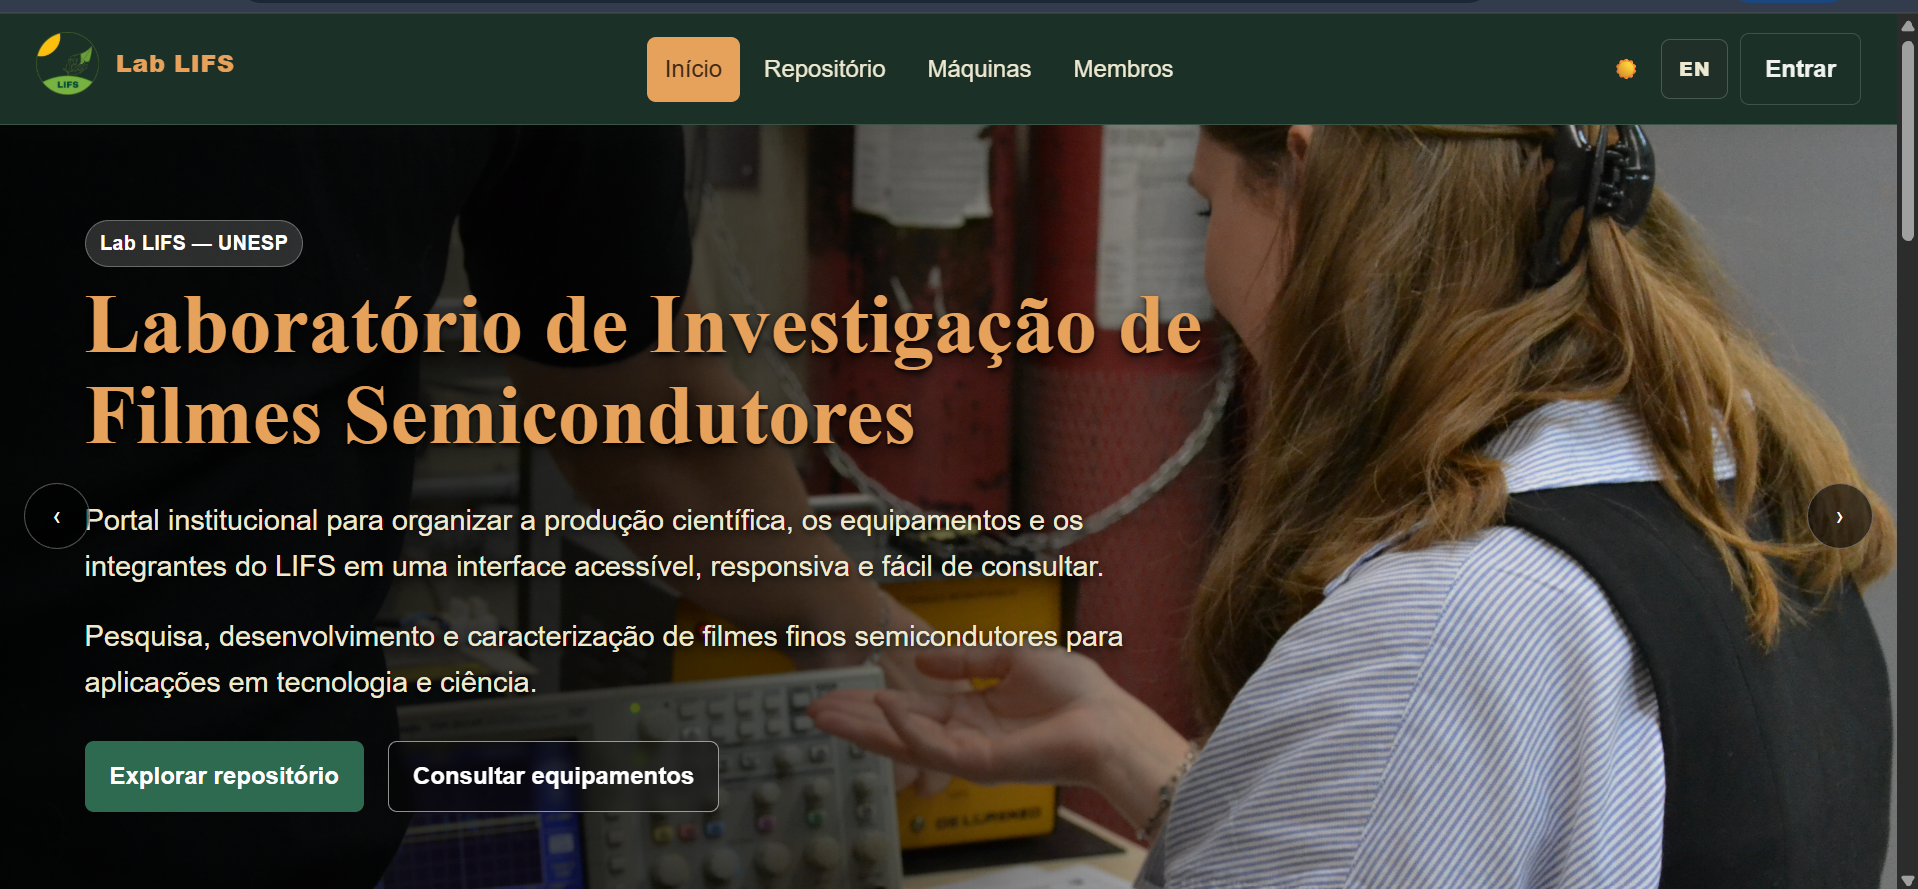
\includegraphics[width=\linewidth]{2-imagens/print_home_dark}
		\caption{Página inicial em tema escuro.}
		\label{fig:home-dark}
	\end{subfigure}
	\hfill
	\begin{subfigure}{0.48\textwidth}
		\centering
		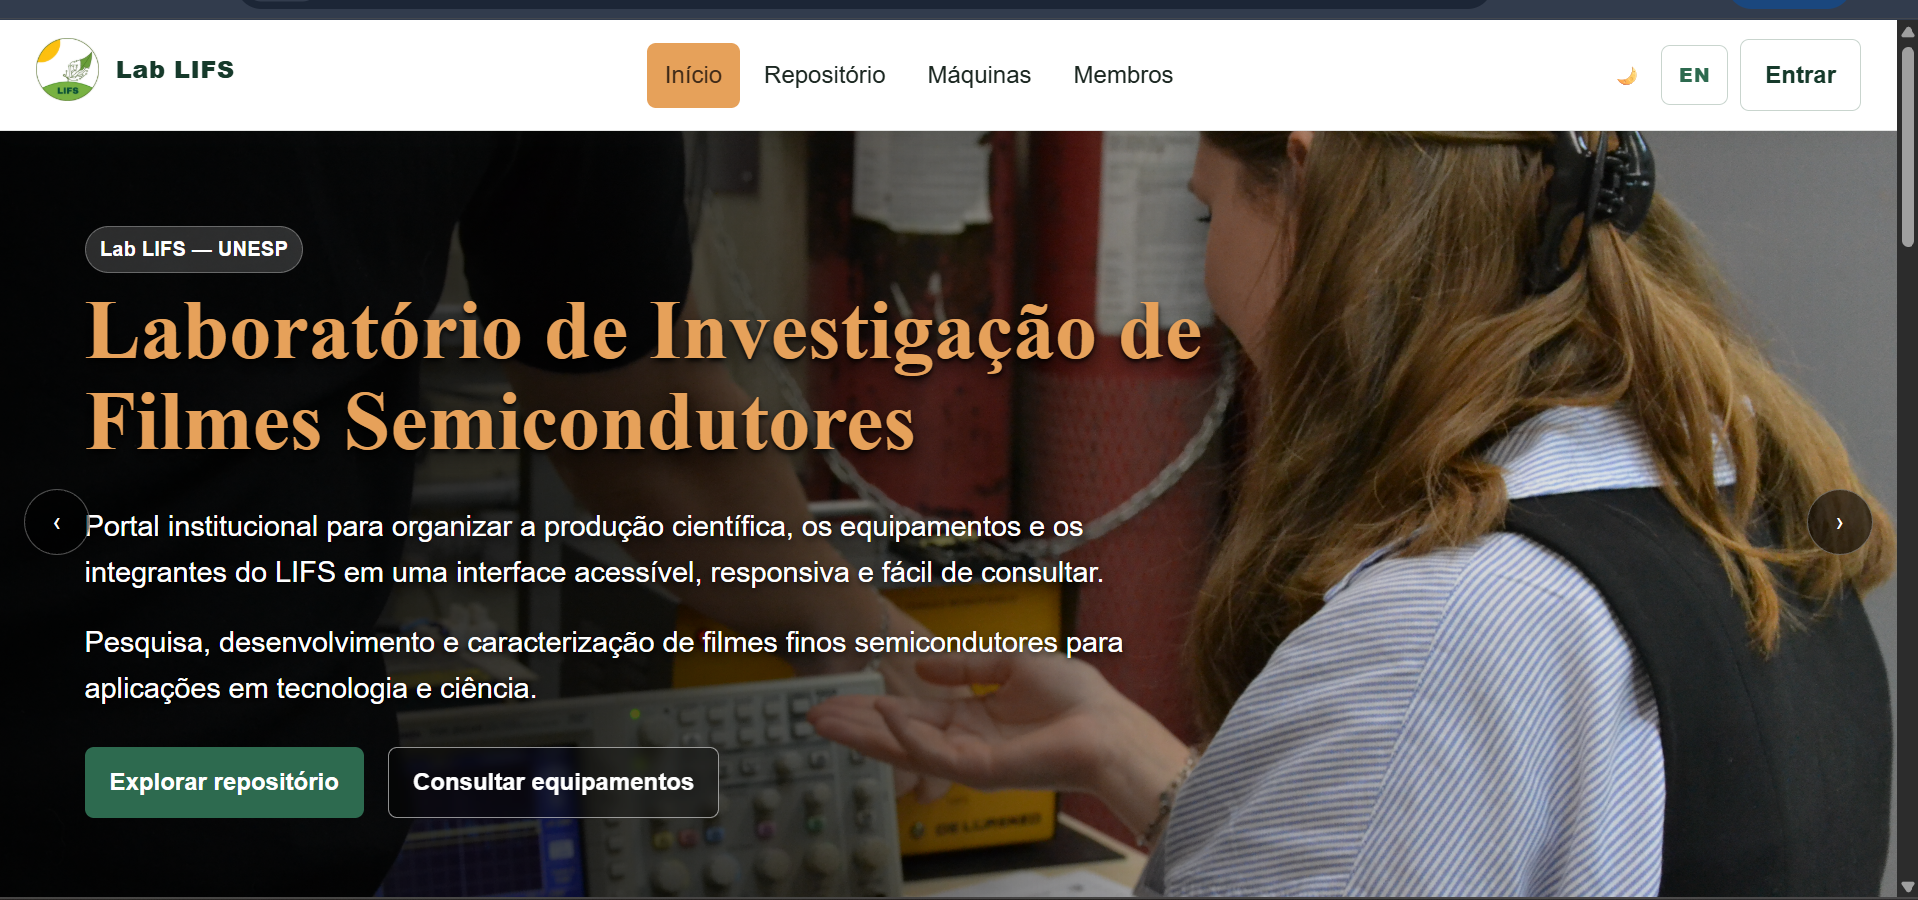
\includegraphics[width=\linewidth]{2-imagens/print_home_light}
		\caption{Página inicial em tema claro.}
		\label{fig:home-light}
	\end{subfigure}
	
	\vspace{0.5cm}
	
	\begin{subfigure}{0.48\textwidth}
		\centering
		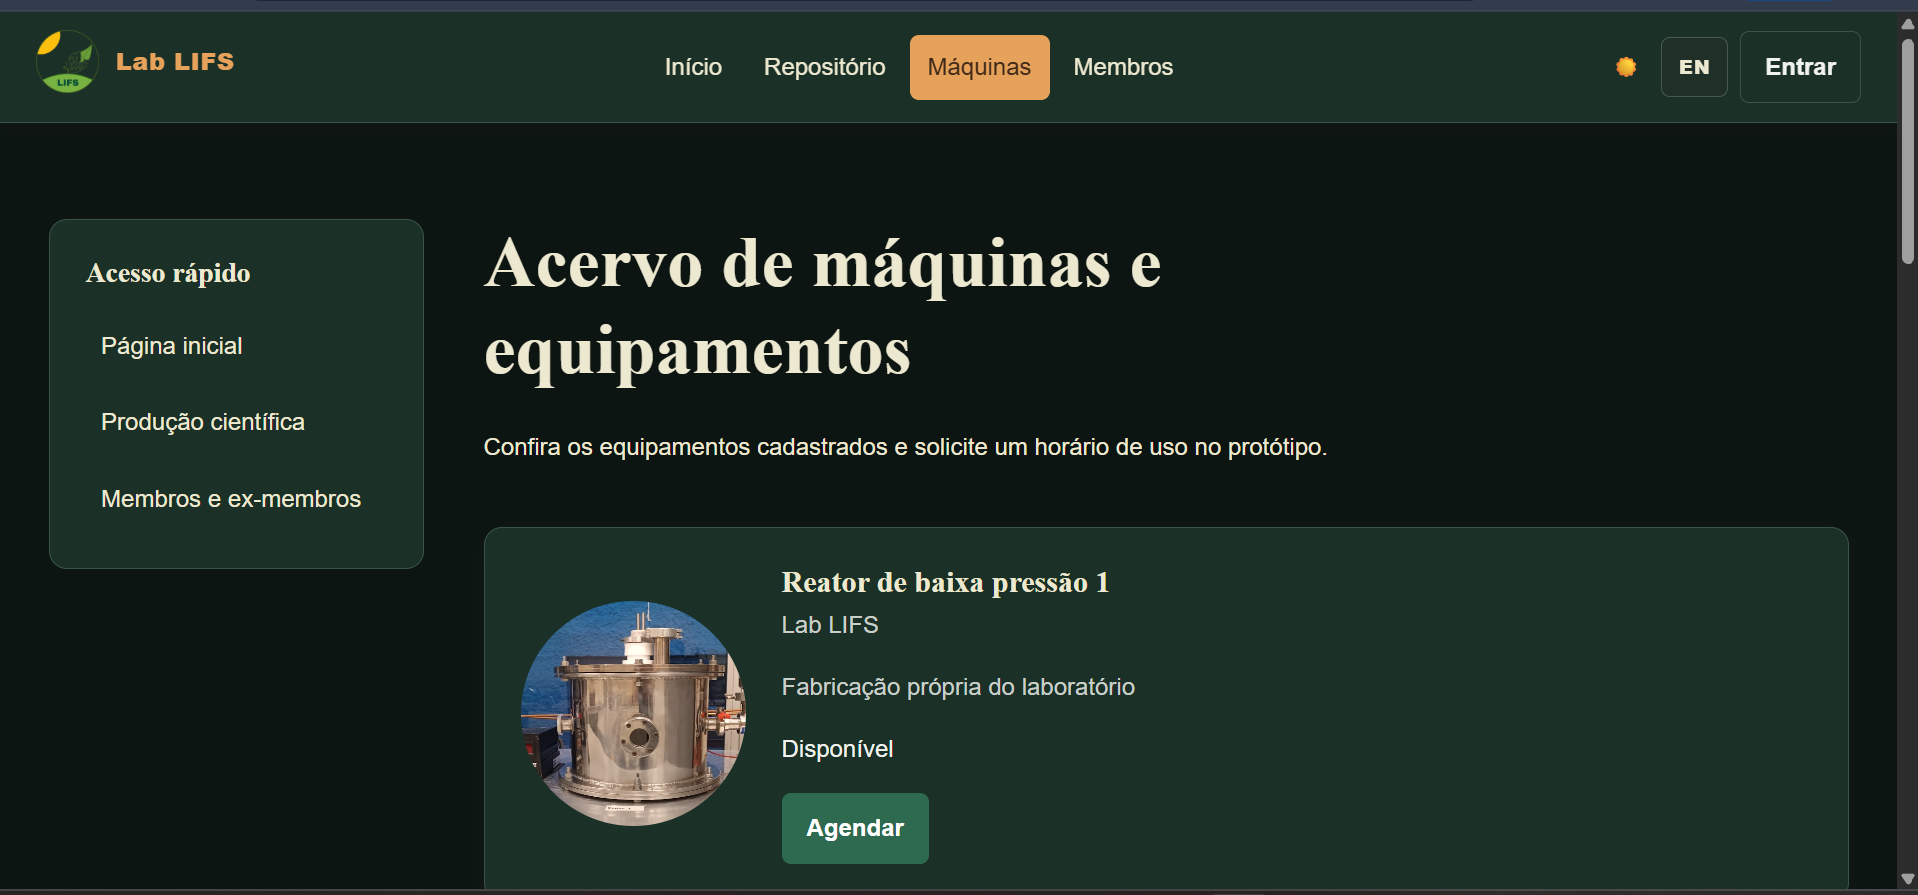
\includegraphics[width=\linewidth]{2-imagens/print_maq_dark}
		\caption{Página de máquinas em tema escuro.}
		\label{fig:maq-dark}
	\end{subfigure}
	\hfill
	\begin{subfigure}{0.48\textwidth}
		\centering
		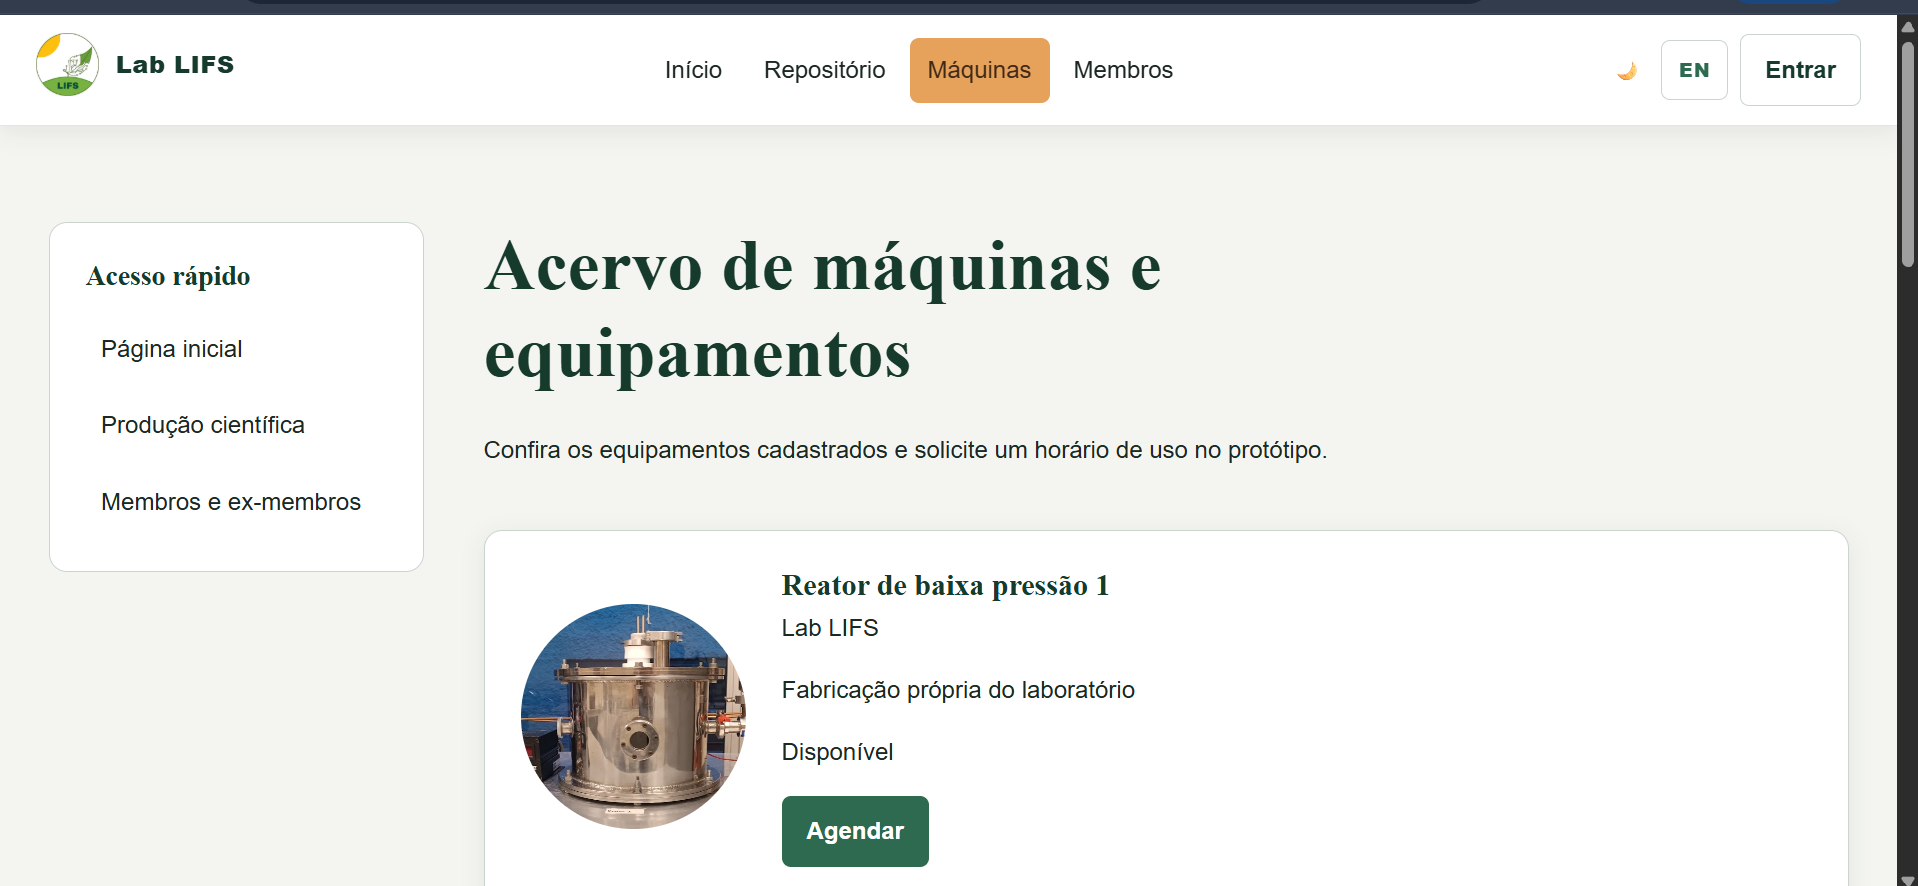
\includegraphics[width=\linewidth]{2-imagens/print_maq_light}
		\caption{Página de máquinas em tema claro.}
		\label{fig:maq-light}
	\end{subfigure}
	
	\caption{Interface do sistema nas páginas inicial e de máquinas, 
		apresentando os temas claro e escuro.}
	\label{fig:interface-temas}
\end{figure}

\subsubsection{User Experience (UX)}

No âmbito da experiência do usuário, a estrutura do sistema foi organizada
a partir da forma como diferentes usuários podem buscar informações sobre um
laboratório de pesquisa. A navegação principal foi dividida em categorias
associadas a conceitos distintos do LIFS, como \textit{Início},
\textit{Membros}, \textit{Máquinas} e \textit{Repositório}.

Essa organização constitui uma forma de arquitetura da informação, na qual
os conteúdos são agrupados segundo sua finalidade e não segundo sua
implementação interna. Assim, um usuário interessado em identificar os
pesquisadores pode acessar diretamente a área de membros, enquanto um
usuário interessado na infraestrutura pode consultar a seção de máquinas.
De maneira semelhante, a produção científica pode ser acessada por meio do
repositório.

A estrutura pode ser representada conceitualmente da seguinte maneira:

\begin{figure}[H]
	\centering
	\begin{tikzpicture}[
		box/.style={
			draw,
			rounded corners=2pt,
			align=center,
			minimum width=2.8cm,
			minimum height=0.8cm
		},
		arrow/.style={
			->,
			thick
		}
		]
		
		% Sistema principal
		\node[box] (lifs) at (0,2.5) {Sistema LIFS};
		
		% Áreas principais
		\node[box] (inicio) at (-5,0) {Início};
		\node[box] (repo) at (-1.7,0) {Repositório};
		\node[box] (maquinas) at (1.7,0) {Máquinas};
		\node[box] (membros) at (5,0) {Membros};
		
		% Funcionalidade do Repositório
		\node[box] (adicionar) at (-1.7,-2) {Adicionar Trabalho};
		
		% Ligações principais
		\draw[arrow] (lifs) -- (inicio);
		\draw[arrow] (lifs) -- (repo);
		\draw[arrow] (lifs) -- (maquinas);
		\draw[arrow] (lifs) -- (membros);
		
		% Ligação do Repositório
		\draw[arrow] (repo) -- (adicionar);
		
	\end{tikzpicture}
	\caption{Organização hierárquica das principais áreas e funcionalidades do sistema LIFS.}
	\label{fig:arquitetura-lifs}
\end{figure}

Além disso, a presença de diferentes perfis de utilização foi considerada
na concepção do sistema. Um visitante externo pode utilizar a plataforma
principalmente para conhecer o laboratório e consultar suas informações,
enquanto um membro do grupo pode necessitar de funcionalidades adicionais,
como o cadastro de trabalhos. Essa diferenciação constitui uma base para a
evolução futura do sistema, especialmente para funcionalidades relacionadas
a autenticação, gerenciamento de conteúdo, disponibilidade de equipamentos e
agendamento.

\subsubsection{Fluxos de interação}

As funcionalidades do sistema também foram organizadas de maneira a
estabelecer relações entre consulta e execução de tarefas. Um exemplo é o
fluxo relacionado ao repositório científico, no qual o usuário pode acessar
os trabalhos disponíveis e, posteriormente, utilizar funcionalidades de
cadastro para inserir novas produções.

De forma conceitual, o fluxo pode ser representado como:

\begin{equation}
	\text{Repositório}
	\rightarrow
	\text{Consulta}
	\rightarrow
	\text{Seleção do trabalho}
	\rightarrow
	\text{Visualização}
\end{equation}

Para usuários autorizados, esse fluxo pode ser expandido para:

\begin{equation}
	\text{Autenticação}
	\rightarrow
	\text{Cadastro}
	\rightarrow
	\text{Validação}
	\rightarrow
	\text{Publicação}
\end{equation}

A mesma abordagem poderá ser aplicada futuramente ao gerenciamento dos
equipamentos. Nesse caso, uma possível evolução da experiência de uso seria
permitir que o usuário selecione um equipamento, consulte sua
disponibilidade, escolha uma data e horário e confirme uma solicitação de
uso. Dessa forma, a interface deixa de ser apenas um meio de apresentação
das informações e passa a atuar como uma camada de interação com os
processos do laboratório.

\subsubsection{Estados e feedback da interface}

Outro aspecto relevante para a experiência do usuário é o fornecimento de
feedback após a execução de ações. Operações como cadastro, alteração ou
exclusão de informações devem apresentar ao usuário um retorno indicando se
a operação foi concluída ou se ocorreu algum erro.

Da mesma forma, situações nas quais não existem dados cadastrados devem ser
representadas por estados vazios informativos, evitando que o usuário
interprete uma área vazia como falha do sistema. Por exemplo, quando não
existirem trabalhos cadastrados no repositório, a interface poderá informar
explicitamente essa condição e apresentar uma orientação sobre a ação que
pode ser realizada.

Esses mecanismos são importantes para estabelecer uma comunicação clara
entre o sistema e o usuário, reduzindo incertezas durante a utilização.

\subsubsection{Responsividade e consistência}

A experiência do usuário também deve ser preservada em diferentes tamanhos
de tela. A interface foi concebida utilizando recursos de CSS que permitem a
adaptação da disposição dos elementos conforme o espaço disponível,
possibilitando sua utilização em computadores, notebooks e dispositivos
móveis.
\begin{figure}[H]
	\centering
	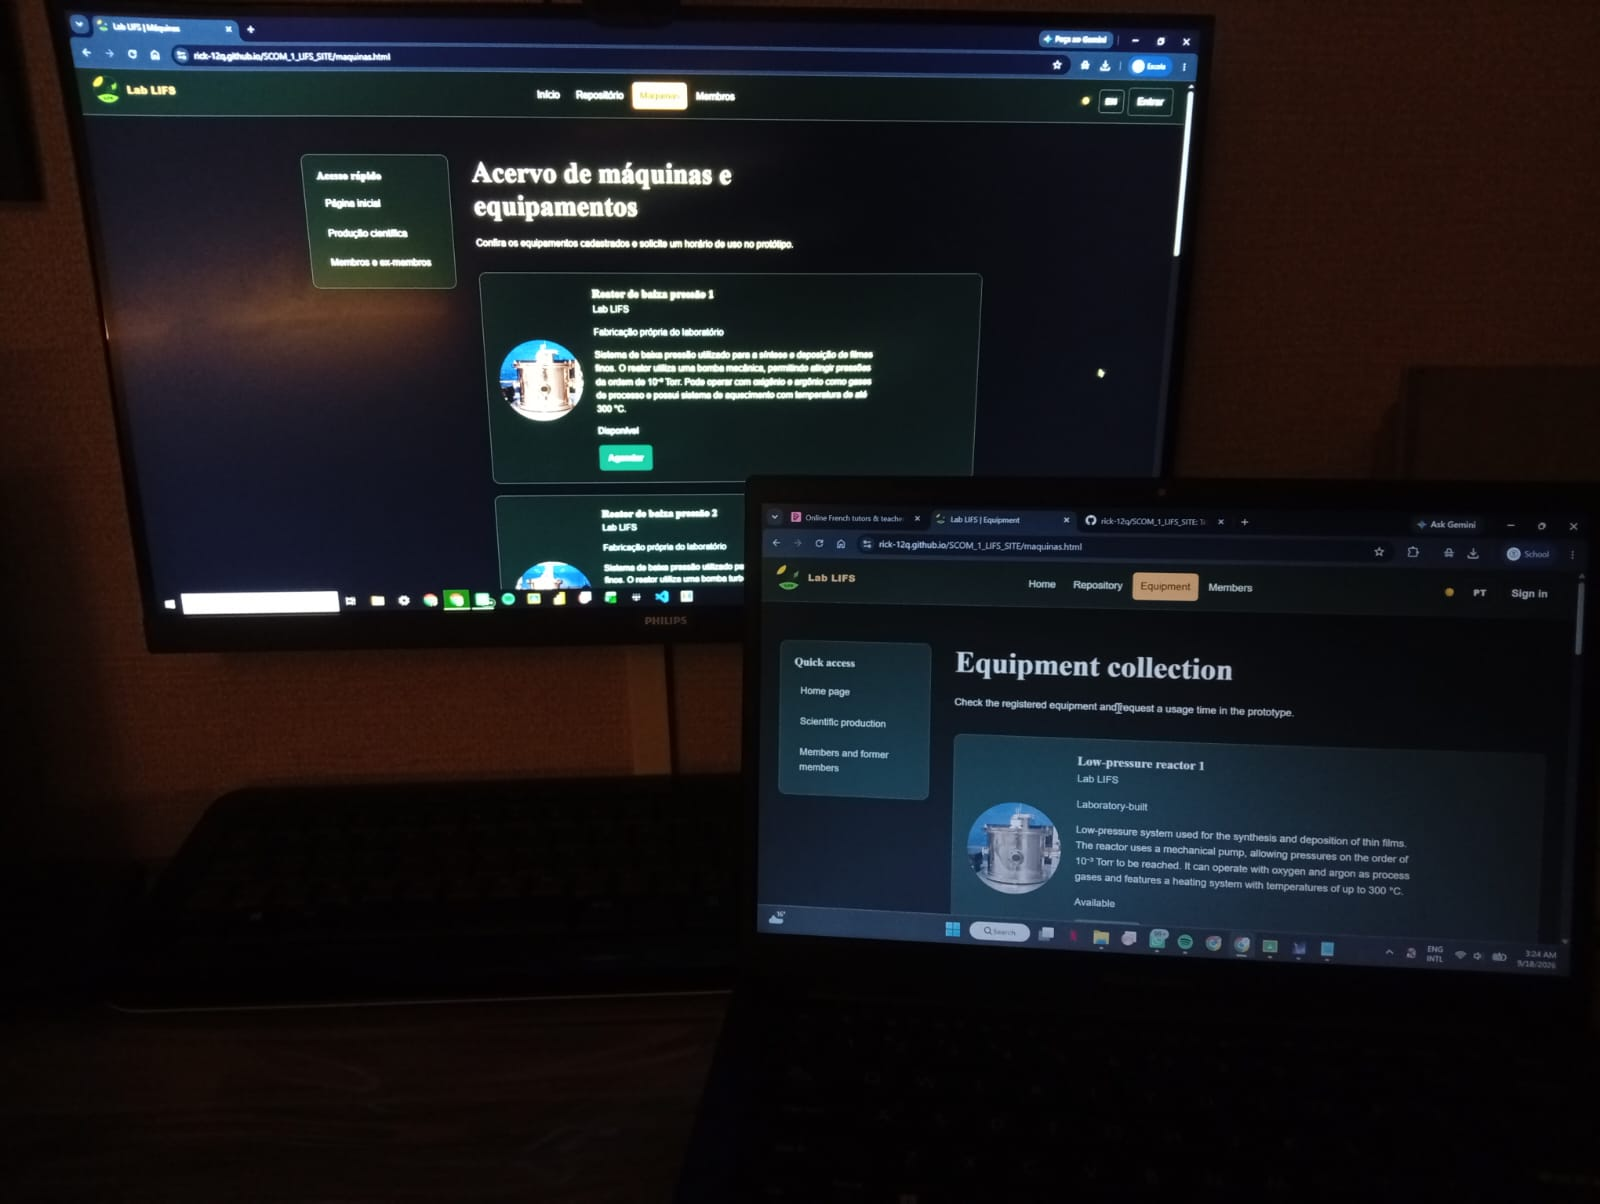
\includegraphics[width=0.7\linewidth]{2-imagens/telas-diferentes}
	\caption{Fotografia de duas telas com tamanhos visivelmente diferentes, enquadrando a mesma página do \textit{website}, evidenciando a responsividade. \\ \centering Fonte: O autor, 2026.}
	\label{fig:telas-diferentes}
\end{figure}

Nesse contexto, responsividade não é considerada apenas como a redução do
tamanho dos elementos, mas como a adaptação da hierarquia e da disposição
das informações. Em telas menores, elementos de navegação e componentes
visuais podem ser reorganizados para preservar sua legibilidade e
acessibilidade.

Dessa maneira, as decisões de UI e UX adotadas no sistema procuram
estabelecer uma relação entre identidade visual, arquitetura da informação e
facilidade de utilização. A interface constitui, portanto, não apenas uma
camada estética do projeto, mas também um mecanismo para organizar e tornar
acessíveis as informações e funcionalidades relacionadas ao LIFS.

	
	%%======%%======%0%======%%=======%%
\vspace{5mm}
\section{Tecnologias utilizadas}


%%======%%======%0%======%%=======%%

A estrutura das páginas foi desenvolvida utilizando \textbf{HTML}, responsável pela organização e definição dos elementos que compõem cada página do sistema, criando assim um esqueleto para o projeto. A utilização de elementos semânticos permitiu estruturar o conteúdo de acordo com sua finalidade, contribuindo tanto para a organização do código quanto para os requisitos relacionados à acessibilidade.

A apresentação visual e a organização dos elementos foram desenvolvidas utilizando \textbf{CSS}. Os arquivos de estilo foram organizados de forma modular, separando diferentes responsabilidades do projeto. Essa organização permitiu estabelecer padrões visuais comuns entre as páginas, além de facilitar a implementação de diferentes disposições para dispositivos com tamanhos de tela distintos.

Para a implementação dos comportamentos interativos da interface foi utilizado \textbf{JavaScript}. A linguagem foi empregada para controlar funcionalidades que dependem de interação do usuário e para modificar dinamicamente determinados elementos da página. Dessa forma, HTML, CSS e JavaScript foram utilizados de maneira complementar, respectivamente, para estruturar, apresentar e proporcionar comportamento à interface.

O desenvolvimento e a organização dos arquivos foram realizados no \textbf{VS Code}, utilizado como ambiente principal de edição. Além do editor, foram utilizadas extensões que auxiliaram o processo de desenvolvimento, incluindo \textit{Prettier}, para formatação do código; \textit{Material Icon Theme}, para organização visual dos arquivos; \textit{Auto Rename Tag}, para facilitar a edição de elementos HTML; e \textit{Live Server}, utilizado para executar e visualizar localmente as páginas durante o desenvolvimento, como ja mencionado na Seção \ref{sec:processo}.

O controle de versão foi realizado por meio do \textbf{Git}, permitindo registrar a evolução do projeto e acompanhar as alterações realizadas durante o desenvolvimento. 

Para a avaliação técnica da interface foram utilizadas ferramentas de análise e validação. O \textbf{Google Lighthouse} foi utilizado para avaliar aspectos relacionados à acessibilidade, desempenho, boas práticas e otimização para mecanismos de busca. A validação da estrutura dos documentos HTML e das folhas de estilo foi realizada por meio dos validadores disponibilizados pelo \textbf{W3C}, permitindo verificar a conformidade dos códigos desenvolvidos com os padrões correspondentes.

	
	\input{1-textos/7-responsividade_acessibilidade}
	
	%%======%%======%0%======%%=======%%
\vspace{5mm}
\section{Resultados dos testes}


%%======%%======%0%======%%=======%%
	
	%%======%%======%0%======%%=======%%
\vspace{5mm}
\section{Compatibilidade de dispositivo}
%%======%%======%0%======%%=======%%

Além da compatibilidade por dimensionamento de tela, ainda é necessário averiguar o funcionamento do \textit{website} em diferentes navegadores, e eventualmente diferentes sistemas operacionais. 

\subsection{Teste de compatibilidade entre navegadores}

A compatibilidade deve ser verificada nos navegadores Google Chrome, Firefox, Edge, Safari e Brave.

Os fluxos principais a serem executados incluem a navegação entre páginas, utilização dos filtros do repositório, abertura dos equipamentos, utilização dos formulários, login, troca de idioma, alteração do tema e utilização do menu em telas menores.

\begin{table}[H]
	\centering
	\caption{Resultados dos testes de compatibilidade entre navegadores.}
	\label{tab:compatibilidade-navegadores}
	\renewcommand{\arraystretch}{1.4}
	\setlength{\tabcolsep}{9pt}
	\begin{tabular}{lcccccc}
		\hline
		\textbf{Fluxo testado} &
		\textbf{Chrome} &
		\textbf{Edge} &
		\textbf{Firefox} &
		\textbf{Safari} &
		\textbf{Brave} &
		\textbf{Opera} \\
		\hline
		Navegação entre páginas & $\checkmark$ & $\checkmark$ & $\checkmark$ & $\checkmark$ & $\checkmark$ & $\checkmark$ \\
		Filtros do repositório & $\checkmark$ & $\checkmark$ & $\checkmark$ & $\checkmark$ & $\checkmark$ & $\checkmark$ \\
		Abertura dos equipamentos & $\checkmark$ & $\checkmark$ & $\checkmark$ & $\checkmark$ & $\checkmark$ & $\checkmark$\\
		Formulários & $\checkmark$ & $\checkmark$ & $\checkmark$ & $\checkmark$ & $\checkmark$ & $\checkmark$ \\
		Login & $\checkmark$ & $\checkmark$ & $\checkmark$ & $\checkmark$ & $\checkmark$ & $\checkmark$ \\
		Troca de idioma & $\checkmark$ & $\checkmark$ & $\checkmark$ & $\checkmark$ & $\checkmark$ & $\checkmark$\\
		Alteração do tema & $\checkmark$ & $\checkmark$ & $\checkmark$ & $\checkmark$ & $\checkmark$ & $\checkmark$\\
		Menu em telas menores & $\checkmark$ & $\checkmark$ & $\checkmark$ & $\checkmark$ & $\checkmark$ & $\checkmark$\\
		\hline
	\end{tabular}
\end{table}

\begin{figure}[H]
	\centering
	
	\begin{subfigure}[t]{0.30\textwidth}
		\centering
		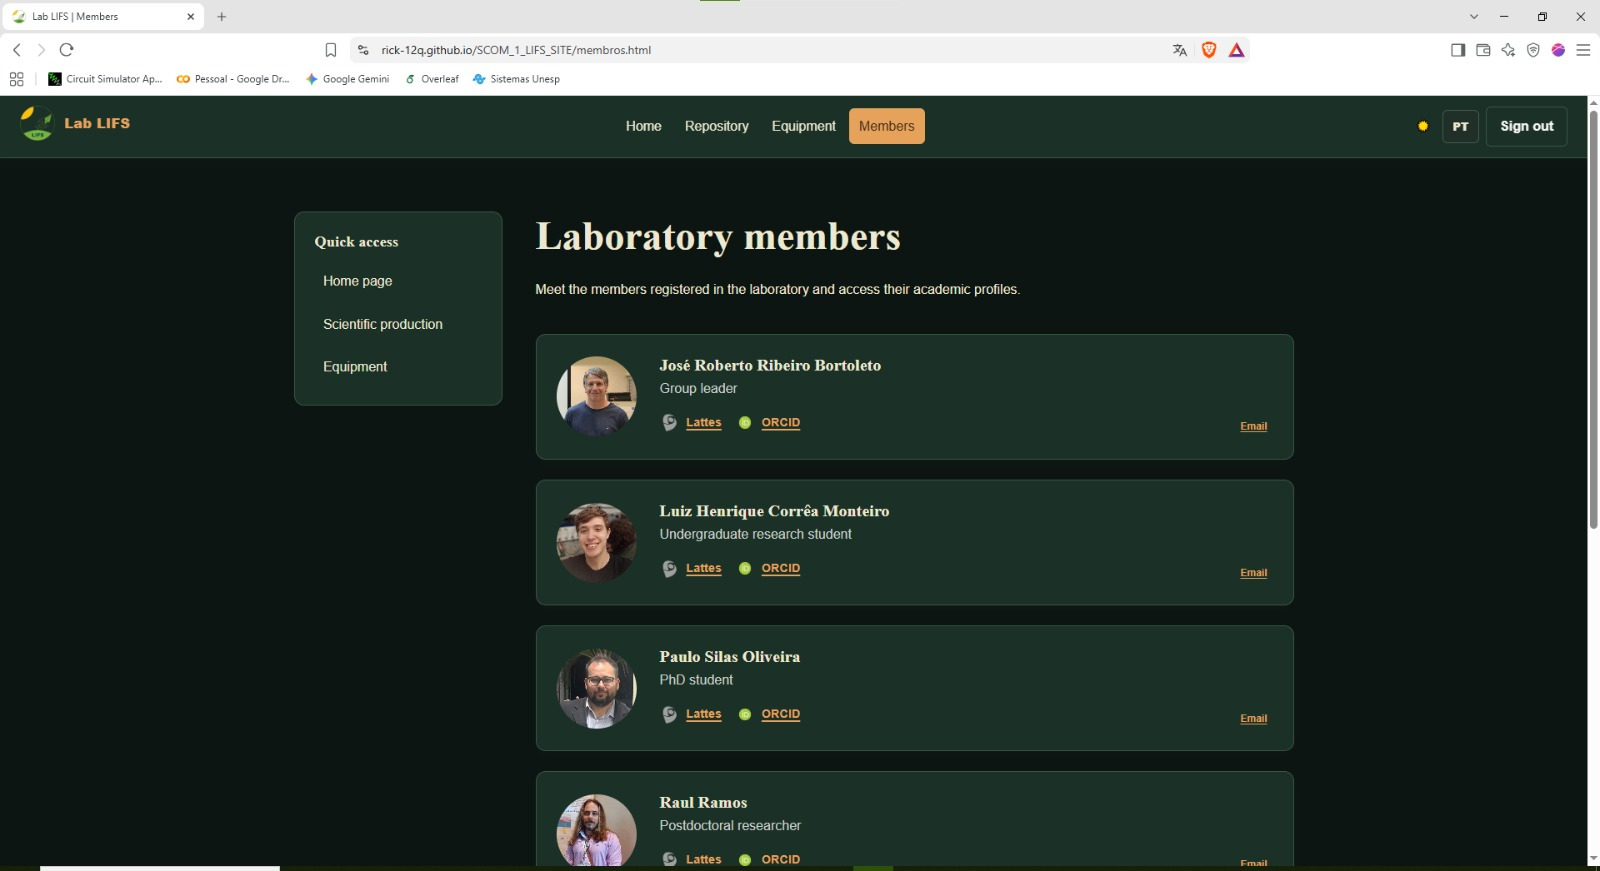
\includegraphics[width=\linewidth,height=0.23\textheight,keepaspectratio]{2-imagens/brave}
		\caption{Brave}
		\label{fig:brave}
	\end{subfigure}
	\hfill
	\begin{subfigure}[t]{0.30\textwidth}
		\centering
		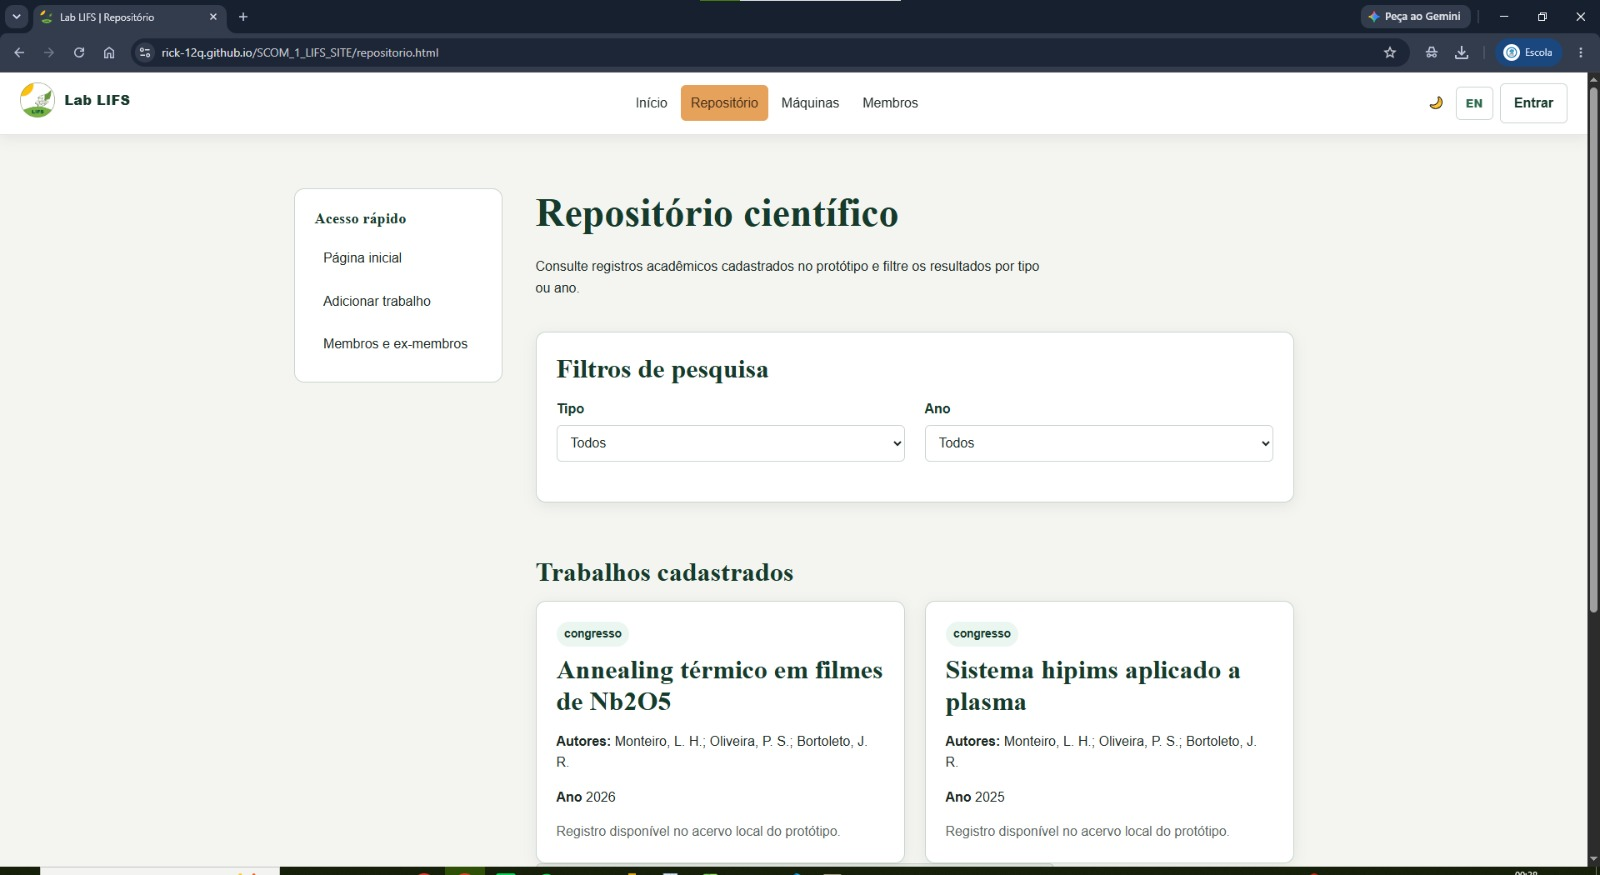
\includegraphics[width=\linewidth,height=0.23\textheight,keepaspectratio]{2-imagens/google}
		\caption{Google Chrome}
		\label{fig:google}
	\end{subfigure}
	\hfill
	\begin{subfigure}[t]{0.30\textwidth}
		\centering
		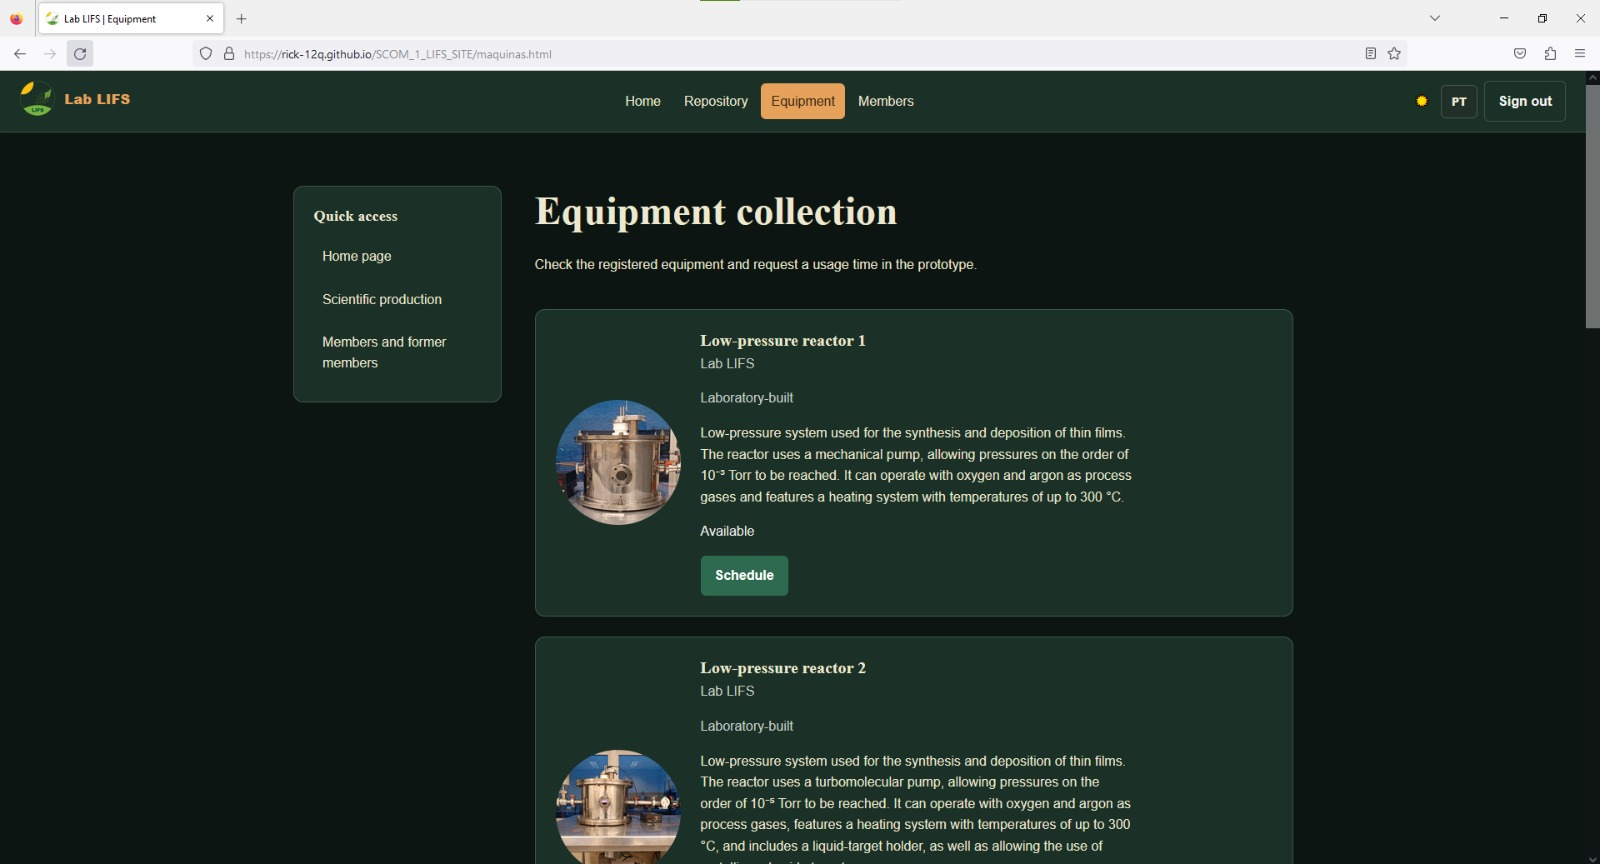
\includegraphics[width=\linewidth,height=0.23\textheight,keepaspectratio]{2-imagens/firefox}
		\caption{Mozilla Firefox}
		\label{fig:firefox}
	\end{subfigure}
	
	\vspace{8mm}
	
	\begin{subfigure}[t]{0.30\textwidth}
		\centering
		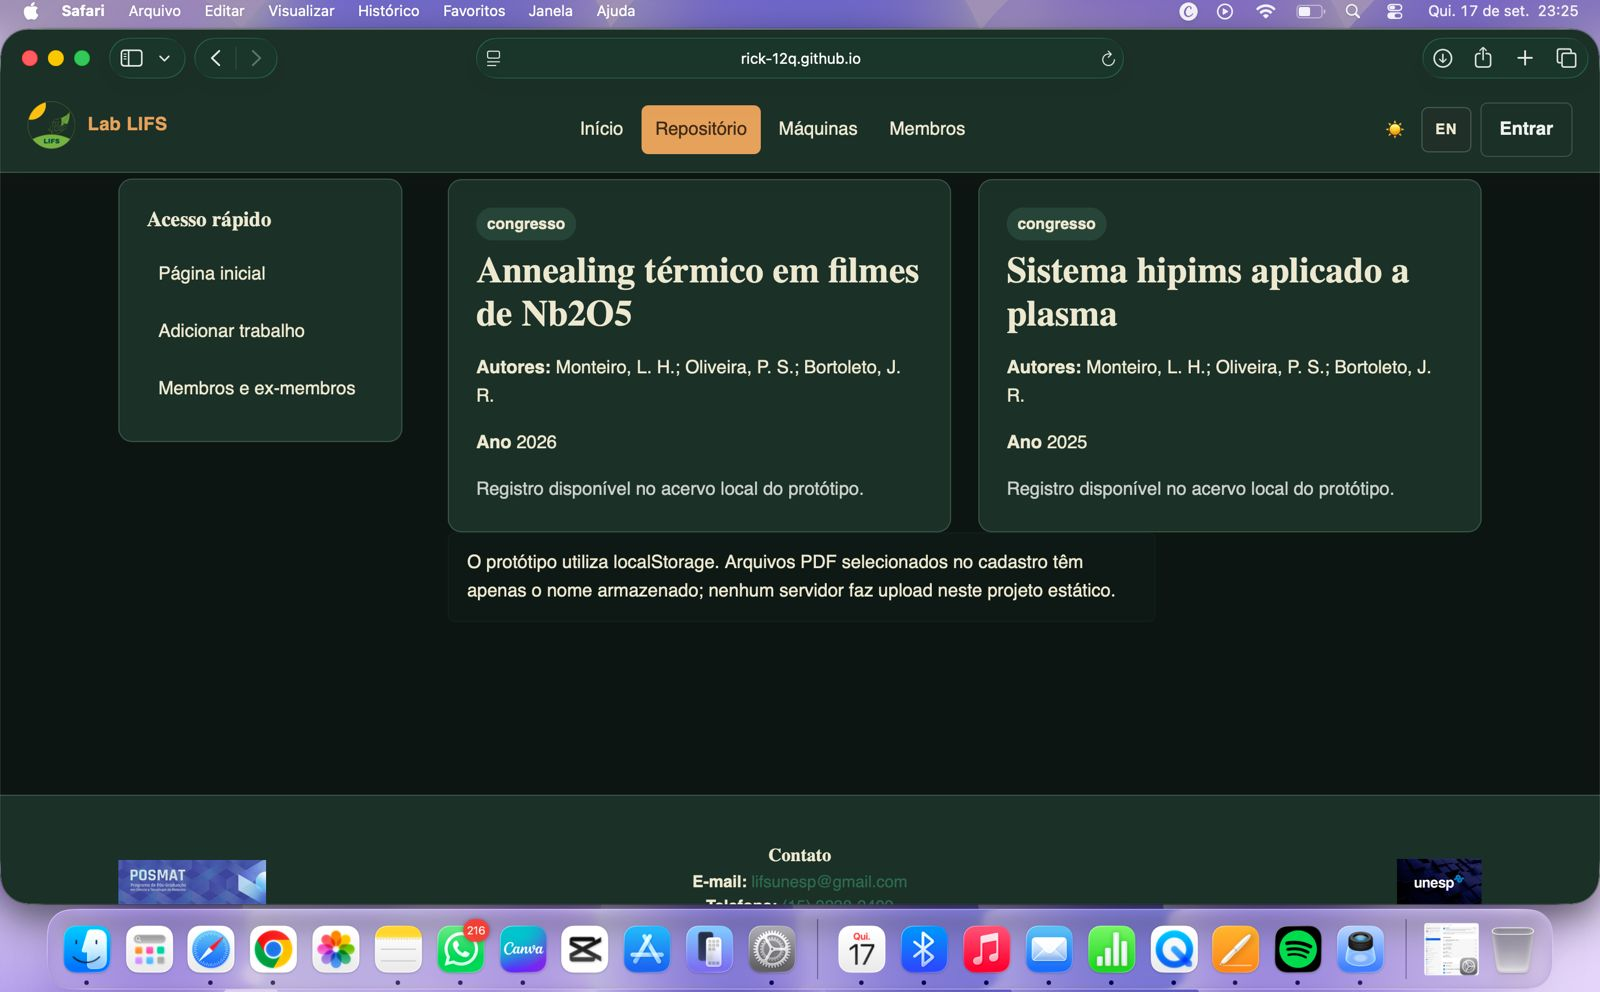
\includegraphics[width=\linewidth,height=0.23\textheight,keepaspectratio]{2-imagens/safari}
		\caption{Safari}
		\label{fig:safari}
	\end{subfigure}
	\hfill
	\begin{subfigure}[t]{0.30\textwidth}
		\centering
		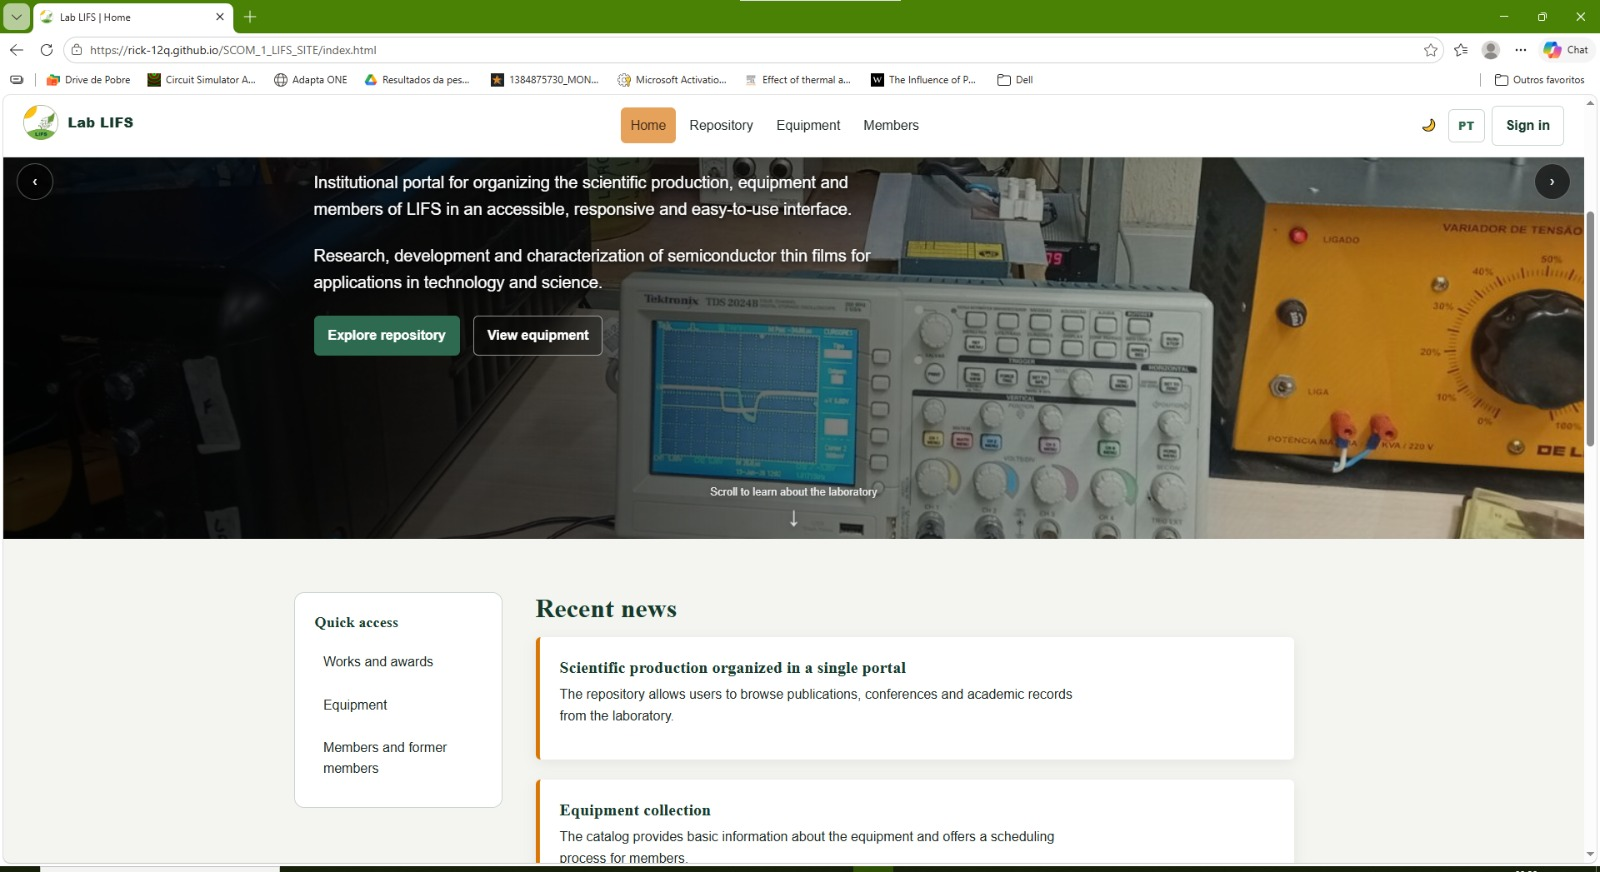
\includegraphics[width=\linewidth,height=0.23\textheight,keepaspectratio]{2-imagens/edge}
		\caption{Microsoft Edge}
		\label{fig:edge}
	\end{subfigure}
	\hfill
	\begin{subfigure}[t]{0.30\textwidth}
		\centering
		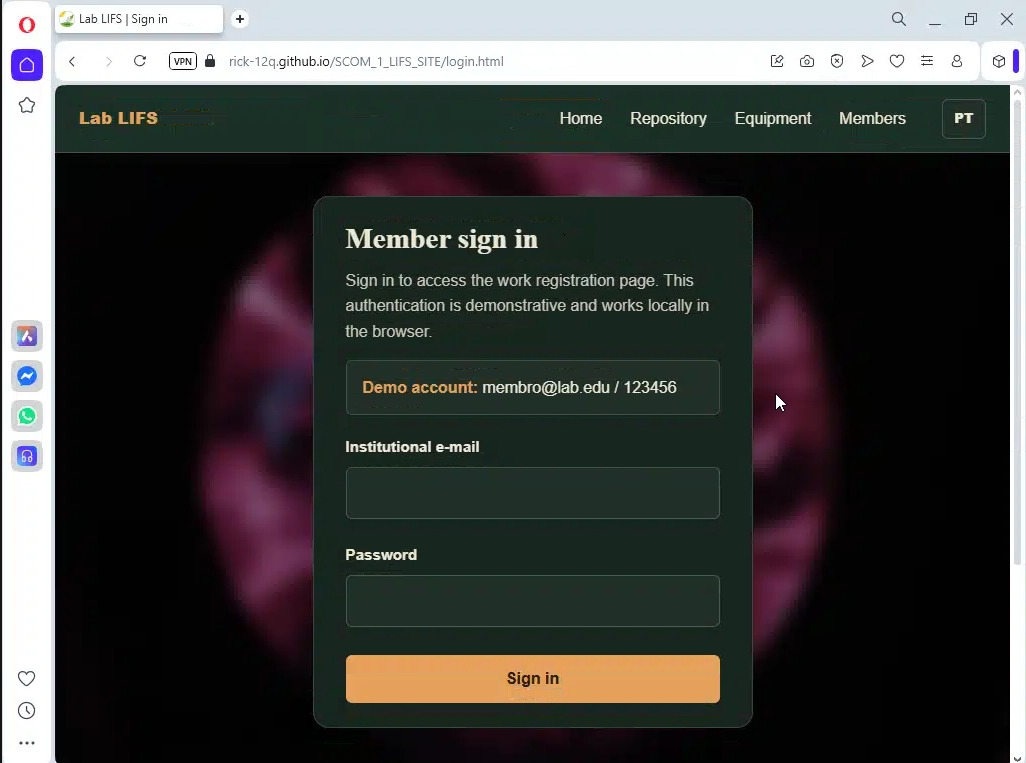
\includegraphics[width=\linewidth,height=0.23\textheight,keepaspectratio]{2-imagens/opera}
		\caption{Opera}
		\label{fig:opera}
	\end{subfigure}
	
	\caption{Testes de compatibilidade do site em diferentes navegadores.\\ \centering Fonte: O autor, 2026.}
	\label{fig:compatibilidade-navegadores}
\end{figure}





	
	%%======%%======%0%======%%=======%%
\vspace{5mm}
\section{Uso de IA generativa}
%%======%%======%0%======%%=======%%

O uso de inteligência artificial foi recorrente no processo de desenvolvimento do trabalho. Especial para a solução de bugs, refinamento de códigos e geração de códigos mais extensos ou complexos. A IA foi utilizada em todos os arquivos de códigos presentes no relatório,e teve maior relevância para o desenvolvimento dos códigos em \texttt{javascript} e \texttt{CSS}, uma vez que estes códigos apresentam maior rigidez, maior complexidade e macetes que são indispensáveis para boas métricas da interface desenvolvida. 

Outro uso relevante de IA no trabalho, foi voltado para a constante validação dos avanços realizados, sendo que a ferramenta, auxiliou o desenvolvimento do projeto fazendo comparações entre a estrutura em desenvolvimento e as exigências do professor referente ao trabalho 1. Desse modo, a IA teve acesso ao código constantemente. 

No que tange ao HTML, a IA trouxe caracteristicas marcantes com o uso de ARIA, ferramentas como o GPT e o CLAUDE inserem com alta frequência o recurso, sendo em alguns momentos, necessário o controle e a reestruturação, prevenindo redundâncias ou excessos por parte do código.

Deve ser ressaltado, que a inteligência artificial (especificamente a ferramenta Claude), desenvolveu um modelo de site, baseado nos preceitos discutidos anteriormente, o qual foi usado como esqueleto principal para o desenvolvimento da interface atual. Porém, elementos como \texttt{javascript} e \texttt{CSS} sofreram alterações quase que totais, uma vez que, ao longo do processo, novas implementações, readequações e certos problemas ou soluções surgiram.

Os códigos, todos, passaram por revisão e refinamento de inteligência artificial, entretanto, os trechos que foram gerados significativamente por IA, estão claramente indicados no código. Destacam-se os arquivos \texttt{components.css}, devido a sua extensão e abrangência, \texttt{i18n.js} devido a sua complexidade, a IA foi especialmente usada para criar a lista de palavras a serem traduzidas e \texttt{adicionar-trabalho.js}, pois foi encontrada uma dificuldade relevante pelo aluno autor de fazer o código funcionar devidamente, vale destacar que o \texttt{README} foi enfeitado pelo Gemini PRO, entretanto o texto ali presente é INTEGRALMENTE escrito pelo aluno autor. Foi apenas corrigido e estruturado mais estéticamente em \texttt{markdown}.

Dessa forma, a inteligência artificial foi utilizada como ferramenta de apoio durante o desenvolvimento, revisão, estruturação e validação do projeto, enquanto as decisões sobre a implementação, alterações no código e adequação às necessidades do trabalho permaneceram sob controle do desenvolvedor. 

Uma tabela (Tabela \ref{tab:uso-ia-arquivos}) mais detalhada pode ser consultado na Seção \ref{sec:apendice}, de apêndices.

	
	%%======%%======%0%======%%=======%%
\vspace{5mm}
\section{Limitação}
%%======%%======%0%======%%=======%%

Apesar de o sistema desenvolvido atender à proposta inicial de apresentar o Laboratório de Investigação de Filmes Semicondutores e organizar suas principais informações, algumas limitações ainda permanecem na versão atual. Isso ocorre principalmente porque o projeto foi desenvolvido dentro do escopo da primeira etapa da disciplina SCOM, que possui como foco a construção e avaliação da interface web. Dessa forma, algumas funcionalidades foram estruturadas apenas até o nível necessário para demonstrar seu funcionamento no protótipo.

Uma das principais limitações está relacionada à persistência dos dados. Parte das informações utilizadas pelo sistema é armazenada por meio do \textit{LocalStorage} do navegador. Essa abordagem é suficiente para o funcionamento de uma aplicação local e para demonstrar o fluxo de cadastro e consulta, porém não representa uma solução adequada para uma utilização simultânea por vários usuários. Os dados permanecem associados ao navegador utilizado e não existe, na implementação atual, uma base de dados central responsável por armazenar e sincronizar as informações.

Essa limitação aparece principalmente no repositório de trabalhos e no gerenciamento das informações apresentadas nas páginas. O sistema já possui uma estrutura para cadastro de trabalhos e organização dos dados, mas ainda não existe uma camada de servidor responsável por validar, armazenar e disponibilizar essas informações de maneira centralizada. Portanto, o cadastro realizado no protótipo não deve ser entendido como um sistema definitivo de gerenciamento da produção científica do laboratório.

A autenticação também possui uma limitação semelhante. Embora exista uma página de login e uma lógica de controle de sessão no lado do cliente, ela ainda não corresponde a um mecanismo de autenticação de usuários adequado para uma aplicação real. Como a aplicação é predominantemente estática e executada no navegador, não existe atualmente um servidor responsável por verificar credenciais e controlar permissões de maneira segura. Assim, essa funcionalidade deve ser considerada parte da estrutura inicial do sistema, e não um controle de acesso definitivo.

Outra limitação está no agendamento dos equipamentos. A página de máquinas já apresenta os equipamentos disponíveis e a interface foi preparada considerando a possibilidade de solicitação de uso, porém o controle efetivo de disponibilidade ainda não está implementado de forma centralizada. Não há, por exemplo, um calendário compartilhado que impeça dois usuários de solicitarem o mesmo equipamento para o mesmo período. Essa parte foi deixada como uma evolução natural do projeto, principalmente porque exigiria uma estrutura de dados persistente e regras para tratamento dos horários.

Também existe uma limitação relacionada aos próprios documentos disponibilizados no repositório. Nem todos os trabalhos científicos podem simplesmente ter seus arquivos PDF disponibilizados publicamente, devido às condições de publicação e aos direitos associados a determinados periódicos. Por esse motivo, uma versão futura do sistema deverá diferenciar a existência do registro bibliográfico da disponibilização do arquivo completo. Em alguns casos, pode ser mais apropriado apresentar os dados da publicação e direcionar o usuário para a fonte oficial.

	
	\vspace{5mm}
\section{Trabalhos futuros}

A evolução mais direta do projeto consiste em transformar a estrutura atual, que funciona principalmente como um protótipo de interface, em uma aplicação com persistência e gerenciamento centralizado dos dados. Para isso, uma das primeiras etapas seria substituir o uso do \textit{LocalStorage} por um banco de dados. Dessa maneira, informações de membros, equipamentos, trabalhos e agendamentos poderiam ser mantidas independentemente do navegador utilizado.

A partir dessa estrutura seria possível implementar um sistema de autenticação propriamente dito. Os usuários poderiam possuir diferentes níveis de acesso, por exemplo, visitantes, membros do laboratório e responsáveis pelo gerenciamento do conteúdo. O visitante continuaria tendo acesso às informações públicas, enquanto usuários autenticados poderiam realizar tarefas como cadastrar trabalhos, alterar informações de equipamentos ou administrar determinados conteúdos.

O sistema de repositório também poderia ser ampliado. Atualmente, a estrutura já considera informações como título, autores, ano, tipo de produção e documentos relacionados. Em uma versão posterior, esses dados poderiam ser armazenados em banco de dados e apresentados por meio de filtros e mecanismos de busca. Também seria possível utilizar links para DOI, páginas de periódicos, anais de congressos ou outros endereços oficiais quando o PDF completo não puder ser disponibilizado.

Outro desenvolvimento importante seria a implementação completa do sistema de agendamento das máquinas. O fluxo previsto para essa funcionalidade é relativamente simples: o usuário selecionaria um equipamento, consultaria sua disponibilidade, escolheria uma data e um horário e então enviaria a solicitação. O sistema poderia verificar automaticamente conflitos de horário e apresentar os períodos já ocupados. A confirmação ou recusa das solicitações também poderia ficar disponível para um usuário responsável pelo laboratório.

Essa funcionalidade poderia ser especialmente útil considerando que a página de máquinas já foi estruturada para apresentar informações dos equipamentos, incluindo descrição, fabricante, modelo, finalidade e características. Assim, o próximo passo não seria criar uma página completamente diferente, mas aproveitar a estrutura existente e acrescentar a parte de controle que ainda não existe.

Outra possibilidade seria melhorar o gerenciamento do conteúdo institucional. Notícias, informações dos membros e registros de equipamentos poderiam deixar de ser definidos diretamente nos arquivos JavaScript e HTML e passar a ser administrados por uma interface própria. Isso reduziria a necessidade de modificar o código sempre que uma informação do laboratório precisasse ser atualizada.

Também seria interessante ampliar os recursos de acessibilidade e realizar novos ciclos de avaliação com o Lighthouse, principalmente após a inclusão de novas funcionalidades. A intenção seria não tratar a acessibilidade como uma etapa encerrada na primeira versão, mas como uma característica que acompanha as alterações do sistema. O mesmo vale para desempenho, especialmente caso o número de imagens, vídeos e registros armazenados aumente.

Em uma etapa posterior, o projeto poderia ainda ser integrado a outros serviços utilizados no ambiente acadêmico, como páginas institucionais, ORCID e Currículo Lattes. A página de membros já apresenta a necessidade de reunir informações acadêmicas e links externos, então uma integração mais estruturada poderia facilitar a atualização desses dados.

Por fim, existe a possibilidade de utilizar o projeto como uma base para uma versão efetivamente utilizada pelo LIFS. Nesse cenário, a interface desenvolvida nesta primeira etapa continuaria sendo aproveitada, mas passaria a funcionar como a camada visual de um sistema com servidor, banco de dados, autenticação e controle de permissões. Dessa forma, o trabalho deixaria de ser somente um site institucional e poderia evoluir para uma ferramenta de apoio às atividades do laboratório.
	
	%%======%%======%0%======%%=======%%
\vspace{5mm}
\section{Conclusão}
%\addcontentsline{toc}{chapter}{Conclusão}

%%======%%======%0%======%%=======%%

Infere-se que a interface foi desenvolvida com sucesso para a etapa vigente. Os testes de desempenho indicaram bom funcionamento da interface. Além disso, o objetivo geral do projeto foi atingido, tanto para termos acadêmicos referentes a disciplina de SCOM, quanto para fins práticos do uso no laboratório da plataforma.

Agora, cabem ás próximas etapas, a implementação de um banco de dados, persistência de dados, e o refinamento de pequenos detalhes ainda em abertos no sistema atual. Além disso, cabe agora, a possibilidade de expandir ainda mais as possibilidades e aplicações do sistema LIFS. 

Por fim, pode se dizer, que a realização deste trabalho, entregou uma interface visualmente agradável, com boas métricas, e uma aplicação real interessante, de modo a tornar as possibilidade ainda mais férteis no que tange ao laboratório, além de ter sido desenvolvida por um aluno, oque transforma a experiência do desenvolvedor e dos usuários que tem o conhecimento de tal fato.
	
	
	% ==========================================================
	%                       REFERÊNCIAS
	% ==========================================================
	
	\nocite{*}
	
	\printbibliography
	
	
	% ==========================================================
	%                        APÊNDICES
	% ==========================================================
	
	%%======%%======%0%======%%=======%%
\newpage
\section{Apêndices}
\label{sec:apendice}
%\addcontentsline{toc}{chapter}{Conclusão}

%%======%%======%0%======%%=======%%
\subsection{Uso de IA}
\begin{longtable}{>{\RaggedRight\arraybackslash}p{0.25\textwidth} >{\RaggedRight\arraybackslash}p{0.24\textwidth} >{\RaggedRight\arraybackslash}p{0.43\textwidth}} \caption{Participação da inteligência artificial generativa no desenvolvimento dos arquivos do site.} \label{tab:uso-ia-arquivos}\\ \hline \textbf{Arquivo do código} & \textbf{Função da IA} & \textbf{Análise geral crítica} \\ \hline \endfirsthead \hline \textbf{Arquivo do código} & \textbf{Função da IA} & \textbf{Análise geral crítica} \\ \hline \endhead \texttt{index.html} & \cellcolor{iaRefinamento}\textbf{Refinamento} & Revisão estrutural e semântica. A IA contribuiu para a organização da página inicial, acessibilidade e estrutura do \textit{landing page}, mas a composição final permaneceu sujeita a ajustes manuais. \\ \hline \texttt{login.html} & \cellcolor{iaRefinamento}\textbf{Refinamento} & Código explicitamente revisado e refinado com IA. A contribuição concentrou-se na estrutura da página, organização dos elementos e integração com os demais recursos do site. \\ \hline \texttt{maquinas.html} & \cellcolor{iaAcessibilidade}\textbf{Acessibilidade} & Uso de elementos semânticos, atributos ARIA e estrutura para diálogos. A IA auxiliou na implementação, mas a adequação ao funcionamento real exigiu integração com JavaScript e CSS. \\ \hline \texttt{membros.html} & \cellcolor{iaAcessibilidade}\textbf{Acessibilidade} & A estrutura emprega recursos de acessibilidade e organização semântica. Não há atribuição explícita de geração no arquivo, portanto a participação específica da IA não é quantificada. \\ \hline \texttt{repositorio.html} & \cellcolor{iaGeracao}\textbf{Geração} & Os filtros de pesquisa possuem auxílio explicitamente atribuído ao ChatGPT. A estrutura foi posteriormente integrada ao restante do sistema e às funções de persistência local. \\ \hline \texttt{adicionar-trabalho.html} & \cellcolor{iaGeracao}\textbf{Geração} & Trecho explicitamente declarado como gerado integralmente por IA. A tradução para o inglês e a adaptação ao funcionamento do projeto foram realizadas manualmente. \\ \hline \texttt{404.html} & \cellcolor{iaSemEvidencia}\textbf{Sem atribuição a IA} & Arquivo simples e predominantemente estrutural. O código disponível foi gerado integralmente por mãos humanas. \\ \hline \texttt{variables.css} & \cellcolor{iaRefinamento}\textbf{Refinamento} & O arquivo registra explicitamente o uso do Gemini Pro para definição e refinamento da abordagem visual, especialmente na organização das variáveis e implementação dos temas. \\ \hline \texttt{reset.css} & \cellcolor{iaSemEvidencia}\textbf{Sem atribuição} & Folha de estilo curta e estrutural. Sua função é normalizar o comportamento dos elementos antes da aplicação dos demais estilos. \\ \hline \texttt{base.css} & \cellcolor{iaCorrecao}\textbf{Correção} & O modo escuro foi explicitamente ajustado com auxílio do ChatGPT após problemas de implementação. A IA atuou principalmente na correção do comportamento visual. \\ \hline \texttt{layout.css} & \cellcolor{iaRefinamento}\textbf{Refinamento} & Responsável pela estrutura global, navegação, cabeçalho, rodapé e comportamento responsivo. O arquivo mostra forte integração com decisões de layout realizadas durante o desenvolvimento. \\ \hline \texttt{components.css} & \cellcolor{iaReestruturacao}\textbf{Reestruturação} & É o arquivo com maior participação de IA. GPT e Claude foram utilizados na elaboração e aprimoramento de grandes trechos, enquanto partes das máquinas e membros foram desenvolvidas manualmente. O próprio código registra dependência significativa da IA. \\ \hline \texttt{adicionar-trabalho.js} & \cellcolor{iaCorrecao}\textbf{Correção} & O código partiu de uma tentativa própria que não funcionava adequadamente e foi posteriormente adaptado com auxílio do GPT. A IA atuou principalmente na correção e adequação da lógica de cadastro. \\ \hline \texttt{auth.js} & \cellcolor{iaReestruturacao}\textbf{Reestruturação} & A lógica de autenticação e persistência da sessão foi reestruturada com auxílio do GPT. O uso de \texttt{localStorage} resolveu problemas de perda de sessão durante navegação e atualização das páginas. \\ \hline \texttt{carrossel.js} & \cellcolor{iaAcessibilidade}\textbf{Acessibilidade} & O GPT auxiliou na lógica de carregamento e navegação do carrossel, enquanto o Gemini Pro foi utilizado no tratamento relacionado à acessibilidade e preferência por redução de movimento. \\ \hline \texttt{data.js} & \cellcolor{iaSemEvidencia}\textbf{Sem atribuição significativa} & Arquivo predominantemente voltado ao armazenamento dos dados iniciais do protótipo. A participação específica da IA na sua elaboração não é relevante, usada apenas para validação. \\ \hline \texttt{i18n.js} & \cellcolor{iaAcessibilidade}\textbf{Internacionalização} & As estruturas de tradução foram geradas com auxílio do GPT, enquanto a lógica de seleção de idioma foi posteriormente reestruturada. Representa uma das maiores contribuições da IA para a expansão funcional do projeto. \\ \hline \texttt{login-carrossel.js} & \cellcolor{iaRefinamento}\textbf{Refinamento} & Responsável pelo comportamento visual do carrossel da página de login. O arquivo apresenta lógica simples e integrada ao CSS, com tratamento da preferência por redução de movimento. \\ \hline \texttt{maquinas.js} & \cellcolor{iaReestruturacao}\textbf{Reestruturação} & O código registra explicitamente o uso de IA para reestruturar a apresentação das imagens dos equipamentos e reduzir redundâncias. A contribuição ocorreu sobre uma lógica já em desenvolvimento. \\ \hline \texttt{membros.js} & \cellcolor{iaRefinamento}\textbf{Refinamento} & Implementa renderização dinâmica, categorias, links acadêmicos e abas. A estrutura é fortemente integrada ao sistema de tradução e aos dados locais, embora não haja atribuição significativa de autoria da IA. \\ \hline \texttt{repositorio.js} & \cellcolor{iaCorrecao}\textbf{Correção} & A IA foi utilizada para fazer o mecanismo de exibição e filtragem funcionar. O código também incorpora \texttt{escapeHtml}, demonstrando preocupação com tratamento seguro do conteúdo inserido no DOM. \\ \hline \texttt{tema.js} & \cellcolor{iaRefinamento}\textbf{Refinamento} & Implementa a alternância entre temas e sua persistência no navegador. A lógica é compacta e integrada às variáveis CSS, permitindo separar a aparência da lógica de controle. \\ \hline \texttt{ui.js} & \cellcolor{iaRefinamento}\textbf{Refinamento} & Controla menu responsivo, estado de expansão e atualização do ano do rodapé. O código demonstra integração entre comportamento visual, navegação e tradução. \\ \hline \texttt{video.js} & \cellcolor{iaRefinamento}\textbf{Refinamento} & Controla reprodução, volume, pausa, reinício e reprodução condicionada à visibilidade do vídeo. A lógica utiliza recursos nativos do navegador e permanece relativamente independente. \\ \hline \end{longtable} \vspace{3mm} \noindent \textbf{Legenda da classificação:} \quad \cellcolor{iaGeracao}\textbf{Geração} \quad \cellcolor{iaCorrecao}\textbf{Correção} \quad \cellcolor{iaRefinamento}\textbf{Refinamento} \quad \cellcolor{iaAcessibilidade}\textbf{Acessibilidade/Internacionalização} \quad \cellcolor{iaReestruturacao}\textbf{Reestruturação} \quad \cellcolor{iaSemEvidencia}\textbf{Sem atribuição}

\subsection{metricas}
\subsubsection{W3C CSS}

\begin{figure}[H]
	\centering
	
	\begin{subfigure}[b]{0.48\textwidth}
		\centering
		\includegraphics[width=\linewidth]{"../2-imagens/W3C CSS/base"}
		\caption{Base}
		\label{fig:w3c-base}
	\end{subfigure}
	\hfill
	\begin{subfigure}[b]{0.48\textwidth}
		\centering
		\includegraphics[width=\linewidth]{"../2-imagens/W3C CSS/components"}
		\caption{Components}
		\label{fig:w3c-components}
	\end{subfigure}
	
	\vspace{5mm}
	
	\begin{subfigure}[b]{0.48\textwidth}
		\centering
		\includegraphics[width=\linewidth]{"../2-imagens/W3C CSS/layout"}
		\caption{Layout}
		\label{fig:w3c-layout}
	\end{subfigure}
	\hfill
	\begin{subfigure}[b]{0.48\textwidth}
		\centering
		\includegraphics[width=\linewidth]{"../2-imagens/W3C CSS/reset"}
		\caption{Reset}
		\label{fig:w3c-reset}
	\end{subfigure}
	
	\vspace{5mm}
	
	\begin{subfigure}[b]{0.48\textwidth}
		\centering
		\includegraphics[width=\linewidth]{"../2-imagens/W3C CSS/variables"}
		\caption{Variables}
		\label{fig:w3c-variables}
	\end{subfigure}
	
	\caption{Resultados da validação dos arquivos CSS utilizando o validador W3C.}
	\label{fig:w3c-css}
\end{figure}

\subsubsection{W3C HTML}

\begin{figure}[H]
	\centering
	
	\begin{subfigure}[b]{0.48\textwidth}
		\centering
		\includegraphics[width=\linewidth]{"2-imagens/W3C HTML/login/login"}
		\caption{Login}
		\label{fig:w3c-html-login}
	\end{subfigure}
	\hfill
	\begin{subfigure}[b]{0.48\textwidth}
		\centering
		\includegraphics[width=\linewidth]{"2-imagens/W3C HTML/maq/maquinas errors"}
		\caption{Máquinas}
		\label{fig:w3c-html-maquinas}
	\end{subfigure}
	
	\vspace{5mm}
	
	\begin{subfigure}[b]{0.48\textwidth}
		\centering
		
\includegraphics[width=\linewidth]{"2-imagens/W3C HTML/memb/membros .png"}
		\caption{Membros}
		\label{fig:w3c-html-membros}
	\end{subfigure}
	\hfill
	\begin{subfigure}[b]{0.48\textwidth}
		\centering
		\includegraphics[width=\linewidth]{"2-imagens/W3C HTML/reposit/repositorio"}
		\caption{Repositório}
		\label{fig:w3c-html-repositorio}
	\end{subfigure}
	
	\caption{Resultados da validação dos arquivos HTML utilizando o validador W3C.}
	\label{fig:w3c-html}
\end{figure}

\subsubsection{webAIM}

\begin{figure}[H]
	\centering
	
	\begin{subfigure}[b]{0.48\textwidth}
		\centering
		\includegraphics[width=\linewidth]{"2-imagens/webAIM/TEMA CLARO/cards"}
		\caption{Cards}
		\label{fig:webaim-claro-cards}
	\end{subfigure}
	\hfill
	\begin{subfigure}[b]{0.48\textwidth}
		\centering
		\includegraphics[width=\linewidth]{"2-imagens/webAIM/TEMA CLARO/texto principal"}
		\caption{Texto principal}
		\label{fig:webaim-claro-principal}
	\end{subfigure}
	
	\vspace{5mm}
	
	\begin{subfigure}[b]{0.48\textwidth}
		\centering
		\includegraphics[width=\linewidth]{"2-imagens/webAIM/TEMA CLARO/texto secundario"}
		\caption{Texto secundário}
		\label{fig:webaim-claro-secundario}
	\end{subfigure}
	\hfill
	\begin{subfigure}[b]{0.48\textwidth}
		\centering
		\includegraphics[width=\linewidth]{"2-imagens/webAIM/TEMA ESCURO/texto principal"}
		\caption{Texto principal}
		\label{fig:webaim-escuro-principal}
	\end{subfigure}
	
	\vspace{5mm}
	
	\begin{subfigure}[b]{0.48\textwidth}
		\centering
		\includegraphics[width=\linewidth]{"2-imagens/webAIM/TEMA ESCURO/texto secundario"}
		\caption{Texto secundário}
		\label{fig:webaim-escuro-secundario}
	\end{subfigure}
	\hfill
	\begin{subfigure}[b]{0.48\textwidth}
		\centering
		\includegraphics[width=\linewidth]{"2-imagens/webAIM/header selecionado"}
		\caption{Cabeçalho}
		\label{fig:webaim-header}
	\end{subfigure}
	
	\caption{Testes de contraste visual realizados com a ferramenta WebAIM para os diferentes elementos e temas da interface.}
	\label{fig:webaim}
\end{figure}

\subsubsection{LightHouse}

\begin{figure}[H]
	\centering
	
	\begin{subfigure}[b]{0.31\textwidth}
		\centering
		\includegraphics[width=\linewidth]{"2-imagens/home lighthouse"}
		\caption{Página inicial.}
		\label{fig:home-lighthouse}
	\end{subfigure}
	\hfill
	\begin{subfigure}[b]{0.31\textwidth}
		\centering
		\includegraphics[width=\linewidth]{"2-imagens/login lighthouse"}
		\caption{Login.}
		\label{fig:login-lighthouse}
	\end{subfigure}
	\hfill
	\begin{subfigure}[b]{0.31\textwidth}
		\centering
		\includegraphics[width=\linewidth]{"2-imagens/maq lighthouse"}
		\caption{Máquinas.}
		\label{fig:maq-lighthouse}
	\end{subfigure}
	
	\vspace{5mm}
	
	\begin{subfigure}[b]{0.31\textwidth}
		\centering
		\includegraphics[width=\linewidth]{"2-imagens/membros lighthouse"}
		\caption{Membros.}
		\label{fig:membros-lighthouse}
	\end{subfigure}
	\hfill
	\begin{subfigure}[b]{0.31\textwidth}
		\centering
		\includegraphics[width=\linewidth]{"2-imagens/repositorio lighthouse"}
		\caption{Repositório.}
		\label{fig:repositorio-lighthouse}
	\end{subfigure}
	
	\caption{Resultados das análises realizadas pelo Lighthouse nas páginas do sistema.}
	\label{fig:lighthouse-resultados}
\end{figure}

\subsection{Check list Boas práticas}

\begin{longtable}{p{3.2cm} p{7.2cm} p{3.0cm}}
	
	\caption{Boas práticas utilizadas no desenvolvimento do site.}
	\label{tab:boas-praticas}
	\\
	
	\toprule
	\textbf{Prática} &
	\textbf{Implementação} &
	\textbf{Arquivo} \\
	\midrule
	\endfirsthead
	
	\toprule
	\textbf{Prática} &
	\textbf{Implementação} &
	\textbf{Arquivo} \\
	\midrule
	\endhead
	
	\midrule
	\multicolumn{3}{r}{Continua na próxima página} \\
	\endfoot
	
	\bottomrule
	\endlastfoot
	
	DOCTYPE HTML5 &
	Utilização da declaração \texttt{doctype} correspondente ao HTML5. &
	\texttt{index.html}, linha 2 \\
	
	Atributo \texttt{lang} &
	Definição do idioma principal da página como português do Brasil por meio do atributo \texttt{lang}. &
	\texttt{index.html}, linha 3 \\
	
	Meta viewport &
	Configuração da área de visualização para adaptação do conteúdo às diferentes dimensões de tela. &
	\texttt{index.html}, linha 6 \\
	
	CSS externo &
	Separação dos estilos em arquivos específicos para reset, variáveis, estilos básicos, layout e componentes. &
	\texttt{index.html}, linhas 21--25 \\
	
	Unidades relativas &
	Utilização de unidades e funções relativas, como \texttt{rem}, porcentagem, \texttt{vw}, \texttt{ch}, \texttt{min()} e \texttt{clamp()}. &
	\texttt{css/}, diversos arquivos \\
	
	Imagens com \texttt{alt} &
	As imagens utilizadas no site possuem o atributo alternativo \texttt{alt}. &
	\texttt{index.html} \\
	
	Dimensões explícitas de imagens &
	As imagens do carrossel possuem dimensões definidas por meio dos atributos \texttt{width} e \texttt{height}. &
	\texttt{index.html}, linhas 116--140 \\
	
	Flexbox e Grid &
	Utilização de Flexbox e CSS Grid para organização dos elementos e estrutura das páginas. &
	\texttt{css/layout.css} \\
	
	Ausência de estilos inline &
	Os estilos são mantidos nos arquivos CSS externos, sem utilização de atributos \texttt{style} diretamente nos elementos HTML. &
	Arquivos HTML e CSS \\
	
	IDs não duplicados &
	Os identificadores utilizados nos elementos das páginas são definidos individualmente. &
	Arquivos HTML \\
	
	Links internos &
	Utilização de links para navegação entre as diferentes páginas que compõem o site. &
	Arquivos HTML \\
	
	Foco visível &
	Utilização de \texttt{:focus-visible} para apresentar uma indicação visual durante a navegação por teclado. &
	\texttt{css/base.css}, linhas 48--52 \\
	
	Contraste &
	Utilização de cores centralizadas nas variáveis CSS para padronização da interface nos diferentes temas. &
	\texttt{css/variables.css} \\
	
	Labels associados aos campos &
	Os campos dos formulários possuem elementos \texttt{label} associados aos respectivos campos por meio dos atributos \texttt{for} e \texttt{id}. &
	\texttt{login.html} e formulários \\
	
	Navegação por teclado &
	Implementação de elementos navegáveis por teclado, incluindo botão de menu, link de salto e indicação visual de foco. &
	\texttt{index.html} e \texttt{css/base.css} \\
	
	Estrutura semântica &
	Utilização de elementos semânticos do HTML, como \texttt{header}, \texttt{nav}, \texttt{main}, \texttt{section} e \texttt{footer}. &
	Arquivos HTML \\
	
	Variáveis CSS &
	Definição de valores reutilizáveis dentro de \texttt{:root}, permitindo centralizar cores e demais propriedades da interface. &
	\texttt{css/variables.css} \\
	
\end{longtable}

\subsection{Histórico git}

\begin{lstlisting}[style=gitstyle,
	caption={Histórico de commits do desenvolvimento do projeto.},
	label={lst:historico-git}]
	* fa5c243 (HEAD -> main, origin/main, origin/HEAD) docs: escrita do relatorio
	* 8872e58 perf: compressao de outras fotos
	* 07e8647 perf: compressao de videos e imagens para aumentar lighthouse
	* fa3e505 Remove métricas do repositório
	* bb9de45 docs: atualiza e adiciona um README V2
	* 1f99cb4 fix: correcao de imagem do quatro pontas
	* dcc5abc style: adicao de um favIcon
	* 9f48717 style: ajustes e melhorias nos botoes clicavies de contato com os membros
	* 64f1b3d feat: adicao de mailto nos membros e alteracao do footer
	* 9cbc549 feat: adiciona comentario sobre as maquinas
	* 04ae87d feat: adiciona campo de nome, inst. e motivacao para agendamentos
	* fd01438 perf: Melhora de perfomance adicionando o load lazy
	* 6d99d60 perf: compressao de fotos e videos - melhorar a performance do lighthouse
	* dd0986d Configura GitHub Pages
	* 5b75d3f ajeitando pjt nas pasta Site E Relatorio
	* 3cee70b mexendo no gitignore p arquivos latex
	* 726c986 update
	* 1e32958 style: Adicao de transicao entre idiomas e temas (claro e escuro) e adicao do logo LIFS
	* 5737548 feat: adicao de video institucional e mapa de localizaçao do lab
	* 72a30da fix:Correçao do auth.js que perdia o status de login + Ajuste de membros nao atualizar o idioma
	* 2dd885d feat: Traduçao das paginas de membros e maquinas V2
	* 460383b feat: Traduçao da pagina de erro 404
	* a23b6a9 feat: Traduçao da pagina de adicionar trabalho
	* e4253ed feat: Traduçao da pagina de login
	* 70481d7 feat: Traduçao da pagina de membros
	* e1e16aa feat: Traduçao das paginas de maquinas e repositorio
	* 678f665 feat: adiçao da traduçao em ingles da pagina HOME/INICIO, para acessibilidade de internacionalizandos.
	* f7c428a chore: cria a pasta js/i18n.js para tradução do site em ingles
	* 353e71b feat: adicao do tema ESCURO e CLARO no site
	* 894860b style: Adicao do carrossel na landingpage no inicio.
	* c2d018a style:adicao de um carrossel de fundo na tela de login. alteracoes em java css e html basicas.
	* 368b76b style: Mudanças relevantes no estilo de membros e maquinas, bem como nas fontes principais
	* b934165 chore: cria a pasta para add trabalho .js
	* 5b86a34 style: correcao de ortografia nas legendas
	* dae911f style:ajuste para imagens serem clicaveis
	* 8d2253d style:imagem das maquinas estilizada
	* 9f99d0a style:Adicao das imagens de membros e maquinas
	* c36fff7 refactor: Codigos HTML refinados por IA e maquinas.js adicionadas
	* 7b10636 feat: ajuste das partes faltantes
	* b3cae9b feat: adiciona pagina e logica de autenticacao de usuarios
	* 93a8197 Feature: Adicao do carrosel de imagens
	* 4561067 STYLE: Adicao de trechos do CSS para layout
	* 5ed7317 STYLE: Adicao de trechos do CSS
	* 097b0d6 feat: estrutura inicial do index.html
	* 8e1a315 docs: add de um pseudo readme
	* daad2b1 chore: cria estrutura de pastas, arquivos vazios e gitignore
	* d111ce8 chore: estrutura inicial do projeto
\end{lstlisting}
	
	
\end{document}
